\documentclass[12pt,a4paper,titlepage,listof=totoc,bibliography=totoc,chapteratlists=0pt]{scrreprt}
\newcommand{\thesislang}{de} % en or de
\newcommand{\thesistitle}{Unseen Obstacles - interaktive VR-Simulation zur Sensibilisierung für Barrierefreiheit}
\newcommand{\department}{IT-Medientechnik} % Replace with your department

\newcommand{\firstauthor}{Linnea Schönbauer}
\newcommand{\secondauthor}{Elisa Kaltenberger}

\newcommand{\duedateen}{April 4, 2025} % due date in English format
\newcommand{\duedatede}{4. April 2025} % due date in German format
\newcommand{\firstsupervisor}{Natascha Rammelmüller}
\newcommand{\secondsupervisor}{Markus Haslinger}
\newcommand{\thirdsupervisor}{Stefan Schraml}

\input{header}

\makeatletter
\def\bstctlcite{\@ifnextchar[{\@bstctlcite}{\@bstctlcite[@auxout]}}
\def\@bstctlcite[#1]#2{\@bsphack
	\@for\@citeb:=#2\do{%
		\edef\@citeb{\expandafter\@firstofone\@citeb}%
		\if@filesw\immediate\write\csname #1\endcsname{\string\citation{\@citeb}}\fi}%
	\@esphack}
\makeatother

\clubpenalty=10000 
\widowpenalty=10000
\displaywidowpenalty=10000
\interfootnotelinepenalty=10000

\title{\thesistitle}
\makeatletter
\@ifundefined{fourthauthor}{
  \@ifundefined{thirdauthor}{
    \author{\firstauthor, \secondauthor}
  }{
    \author{\firstauthor, \secondauthor, \thirdauthor}
  }
}{
  \author{\firstauthor, \secondauthor, \thirdauthor, \fourthauthor}
}
\makeatother

\makeindex
\makeglossaries
\begin{document}
\bstctlcite{IEEEexample:BSTcontrol}
\newcommand{\reminder}[1]
{ \textcolor{red}{<[{\bf\marginpar{\mbox{$<==$}} #1 }]>} }
\newcommand{\icode}[1]{\lstinline$#1$}
%\urlstyle{same}
%\setstretch{1.5}
\setstretch {1.433}
\renewcommand{\arraystretch}{1.2}

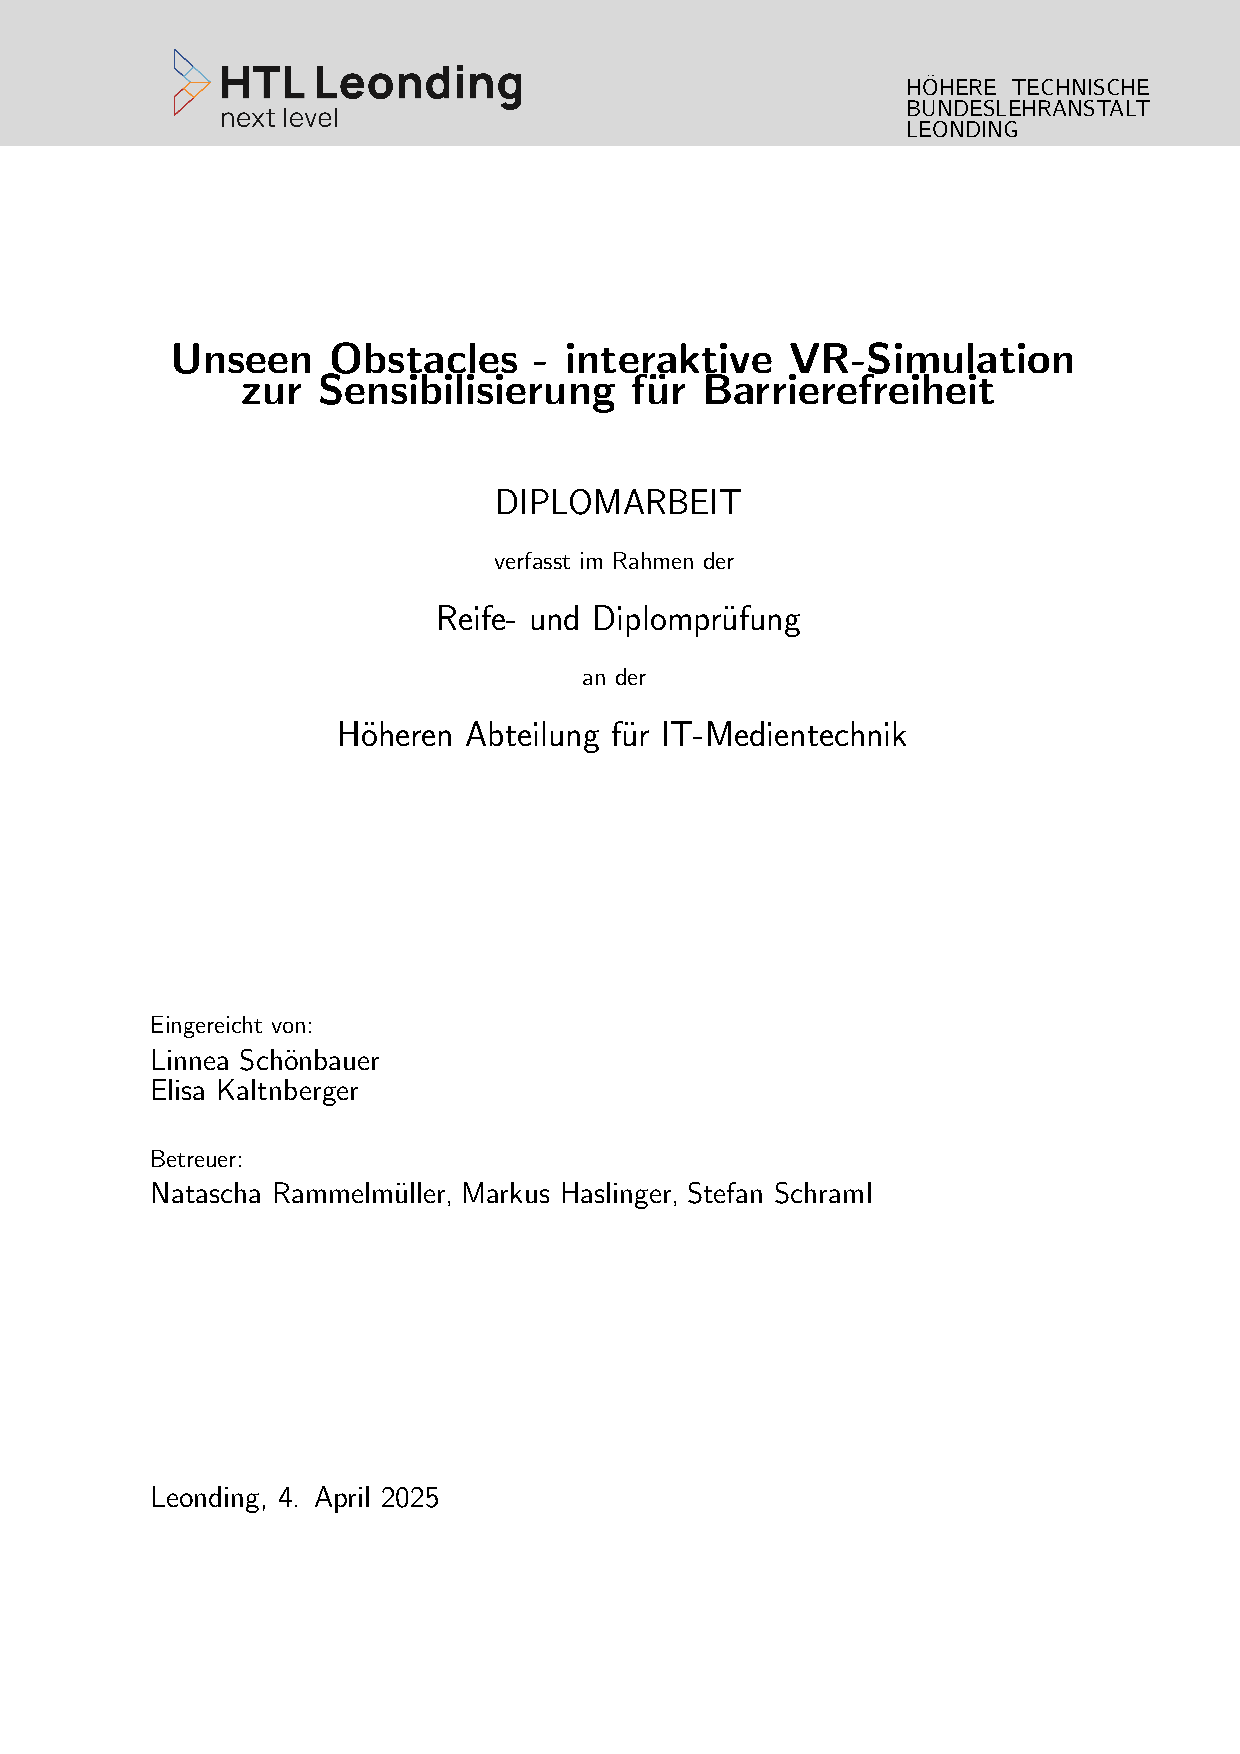
\includepdf{./titlepage/coversheet}
\pagenumbering{Roman}
\newpage
\input{oath}
\begin{spacing}{1}
    \chapter*{Abstract}
\end{spacing}
\begin{wrapfigure}{r}{0.3\textwidth}
    \begin{center}
      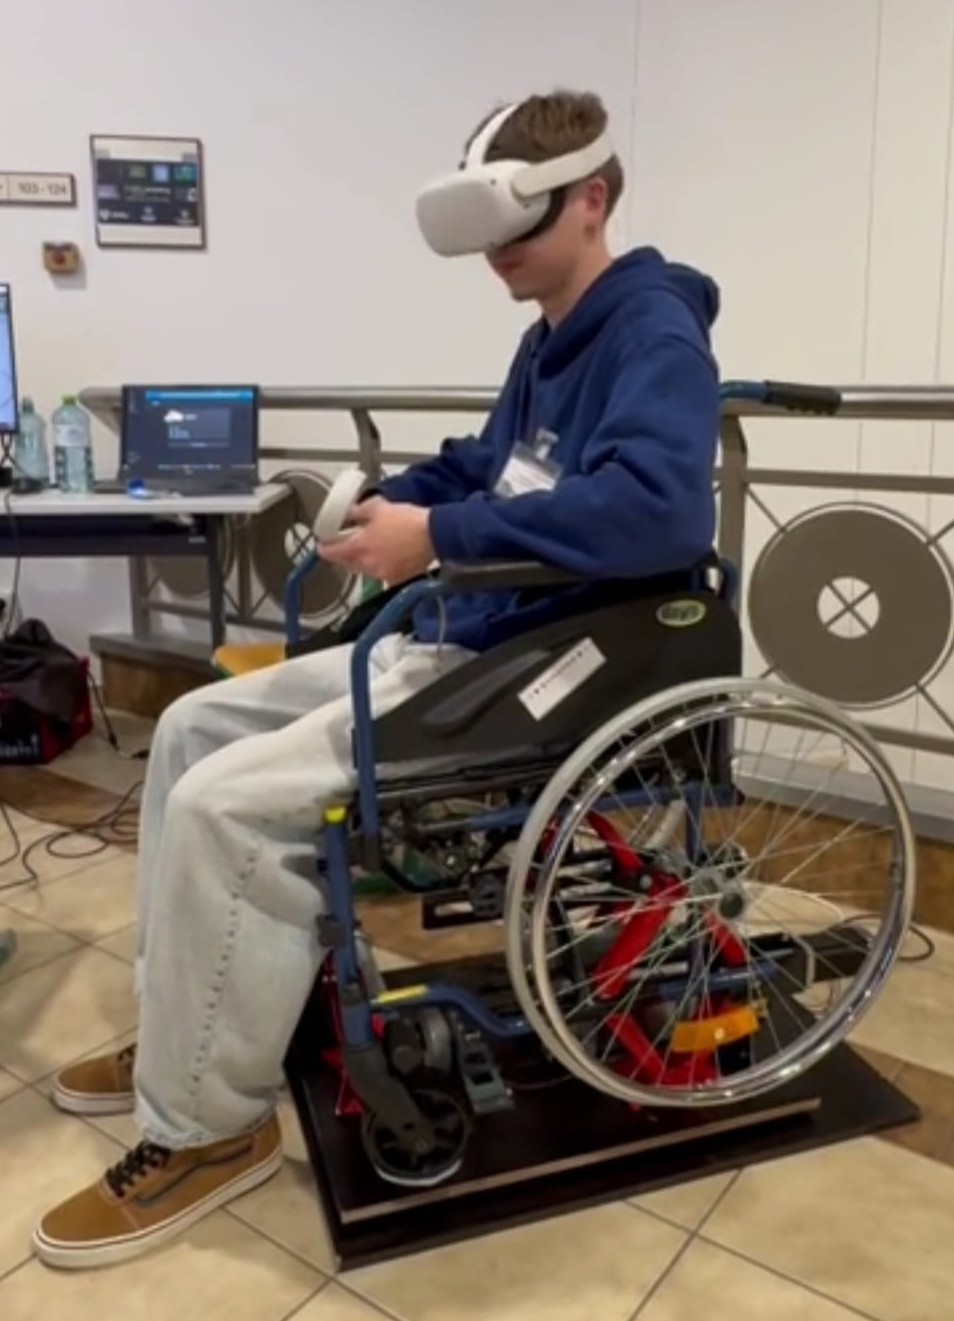
\includegraphics[width=0.4\textwidth]{pics/tdot.jpg}
    \end{center}
\end{wrapfigure}
This thesis investigates how immersive virtual reality (VR) applications can be used to make barriers to wheelchair mobility in urban environments tangible and to raise awareness of the challenges faced by wheelchair users. On the one hand, the focus is on designing a realistic 3D world and facilitating interaction within the virtual environment. On the other hand, a hardware simulator is developed to replicate wheelchair movements.

To this end, a VR environment was created that depicts typical everyday situations, such as navigating streets or overcoming curbs that are too high. In addition, a movable simulator was designed that, in combination with a real wheelchair, provides physical feedback such as tilting and vibrations. This enhances the virtual experience with haptic sensations, making it more realistic.

The results show that the combination of virtual and physical simulation can create a particularly immersive user experience that goes beyond conventional VR applications. Furthermore, the developed solution helps to foster understanding of existing barriers and can be used as a tool for awareness-raising, training, and planning accessible infrastructure.

\newpage
\begin{spacing}{1}
    \chapter*{Zusammenfassung}
\end{spacing}
\begin{wrapfigure}{r}{0.3\textwidth}
    \begin{center}
      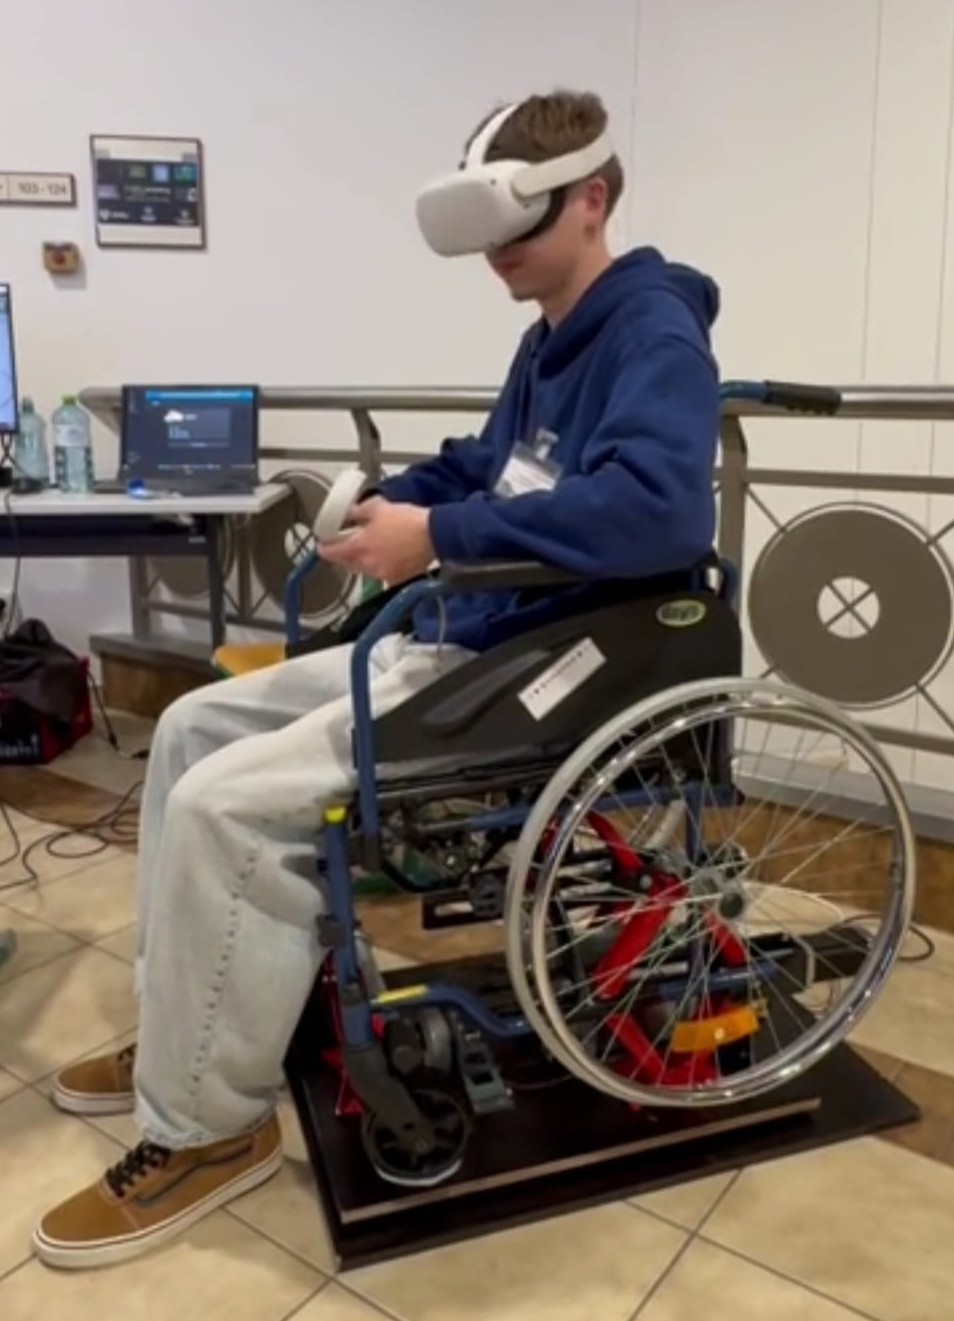
\includegraphics[width=0.4\textwidth]{pics/tdot.jpg}
    \end{center}
\end{wrapfigure}
Die vorliegende Arbeit untersucht, wie immersive Virtual-Reality-Anwendungen genutzt werden können, um Barrieren für die Fortbewegung im Rollstuhl im urbanen Umfeld erfahrbar zu machen und ein Bewusstsein für die Herausforderungen von Rollstuhlfahrenden zu schaffen. Zum einen liegt der Fokus auf der Gestaltung einer realistischen 3D-Welt sowie der Interaktion in der virtuellen Realität. Zum anderen wird ein Hardware-Simulator entwickelt, der Bewegungen im Rollstuhl simuliert.

Hierzu wurde eine VR-Umgebung geschaffen, die typische Alltagssituationen wie das Navigieren durch Straßen oder das Überwinden von zu hohen Bordsteinen abbildet. Ergänzend dazu wurde ein beweglicher Simulator konzipiert, die in Kombination mit einem realen Rollstuhl physische Rückmeldungen wie Neigungen und Vibrationen erzeugt. Dadurch wird die virtuelle Erfahrung durch haptische Eindrücke erweitert und realistischer gestaltet.

Die Ergebnisse zeigen, dass durch die Verbindung von virtueller und physischer Simulation ein besonders intensives Nutzererlebnis erzeugt werden kann, das über klassische VR-Anwendungen hinausgeht. Zudem trägt die entwickelte Lösung dazu bei, das Verständnis für bestehende Barrieren zu fördern und kann als Werkzeug für Sensibilisierung, Ausbildung und die Planung barrierefreier Infrastrukturen eingesetzt werden.


\pagestyle{plain}

\IfStrEq{\thesislang}{de}
{
	\renewcommand{\lstlistlistingname}{Quellcodeverzeichnis}
}
{
 % keep at list of listing
}

\tableofcontents
\newpage
\setcounter{RPages}{\value{page}}
\setcounter{page}{0}
\pagenumbering{arabic}
\pagestyle{scrheadings}

\begin{spacing}{1}
\chapter{Einleitung}\label{chapter:introduction}
\end{spacing}
\setauthor{Elisa Kaltenberger}

Für einen Großteil der Bevölkerung stellt das Treppensteigen eine alltägliche Selbstverständlichkeit dar. 
Diese Selbstverständlichkeit erweist sich für einen geringen Anteil der Einwohner als nicht oder nur bedingt realisierbar. 
Menschen mit körperlichen Einschränkungen sehen sich im Alltag mit signifikanten Herausforderungen konfrontiert. 
Barrieren, die für andere kaum auffallen, können sich als unüberwindbare Hindernisse erweisen. Eine eingeschränkte 
Zugänglichkeit zu Infrastruktur und Dienstleistungen, wie beispielsweise ein nicht erreichbarer Geldautomat aufgrund eines
zu hohen Sichtschutzes oder das Fehlen eines Aufzugs oder einer Rampe, kann die Mobilität enrom einschränken und den 
Alltag erheblich erschweren. Der Fokus liegt dabei nicht ausschließlich auf Mobilität, sondern auch auf der gleichberechtigten 
Teilhabe am gesellschaftlichen Leben.

\section{Statistik}
In Österreich leben rund 1.9 Millionen Menschen im Alter zwischen 15 und 89 Jahren mit gesundheitlichen oder altersbedingten 
Einschränkungen. Dies entspricht etwa einem Viertel der Bevölkerung in dieser Altersgruppe. Die vorliegende Untersuchung 
Abb. \ref{fig:statistik-1}, 
befasst sich mit der Frage, inwiefern die genannte Personengruppe im Alltag von den Auswirkungen betroffen ist. Etwa 
7,6\% der Interviewten gaben an, dass sie sich bei typischen Aktivitäten wie Ankleiden, Einkaufen oder Haushaltsarbeiten durch
starke gesundheitliche Beeinträchtigungen erheblich eingeschränkt fühlen. Rund 17,5\% der Befragten berichteten zumindest eine
leichte Einschränkung.

Dies veranschaulicht, dass Einschränkungen im Alltag ein breites Spektrum umfassen - von leichten Beeinträchtigungen bis hin
zu Situationen, in denen selbst grundlegende Tätigkeiten ohne Hilfe kaum möglich sind. Eine Analyse der Gruppenzusammensetzung 
macht diese Tatsache besonders deutlich. Etwa 30,3\% der österreichischen Bevölkerung mit Behinderungen sind beeinträchtigt.

Die präsentierten Zahlen verdeutlichen, dass Barrierefreiheit und Unterstützungsangebote nicht als Randthema betrachtet
werden können, sondern für einen signifikanten Anteil der Einwohnerschaft von großer Bedeutung sind. Dabei geht es 
nicht nur um Mobilität oder medizinische Versorgung, sondern um die Möglichkeit, das eigene Leben selbstbestimmt zu gestalten 
und gleichberechtigt an der Gesellschaft teilzuhaben. In Anbetracht des demografischen Wandels wird die Relevanz 
barrierefreier Strukturen und inklusiver Maßnahmen in den kommenden Jahren deutlich ansteigen.

\begin{figure}
    \centering
    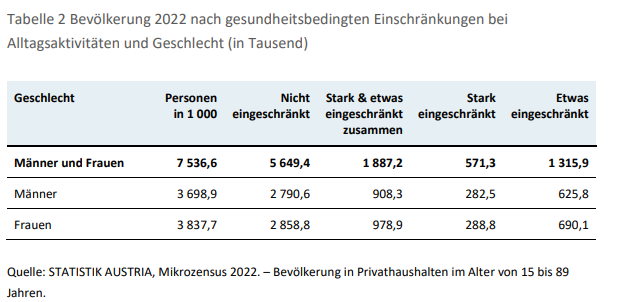
\includegraphics[scale=1]{pics/Statistik-Einschraekungen.png}
    \caption{Statistik Einschraekungen}
    \label{fig:statistik-1}
\end{figure}

Die folgende Tabelle Abb.  \ref{fig:statistik-2} präsentiert die Verteilung gesundheitlicher Einschränkungen bei Alltagsaktivitäten 
in Österreich im Jahr 2022, differenziert nach der Hauptaktivität. Insgesamt geben rund 75\% der Menschen zwischen 15 und 89 
Jahren an, keine Beeinträchtigungen zu haben, während etwa ein Viertel zumindest leichte oder starke Einschränkungen erlebt. 
Diese Korrelation verdeutlicht, dass physische Herausforderungen für einen signifikaten Anteil der Bevölkerung von Relevanz sind.

Bei den Erwerbstätigen und Lehrlingen, die mit rund 55\% die größte Gruppe bilden, sind ungefähr 63\% ohne Einschränkung. 
Etwa 31\% der Teilnehmenden geben an, von leichten oder stärkeren Beeinträchtigungen betroffen zu sein, wobei circa 13\% von 
ihnen starke Beeinträchtigungen verspüren. Dies veranschaulicht, dass trotz körperlicher Herausforderungen ein signifikanter 
Prozentsatz der Gesellschaft einer Erwerbstätigkeit nachgeht.

Arbeitssuchende und Arbeitslose repräsentieren rund 4,4\% der Gesamtbevölkerung in Österreich. Der Anteil der Befragten mit 
starken Einschränkungen liegt hier bei knapp 6\%. Eine ähnliche Entwicklung ist bei dauerhaft arbeitsunfähigen Individuen zu 
beobachten, von denen etwa 16,5\% starke Einschränkungen angeben.

Die Gruppe der Pensionisten, die beinahe ein Viertel der Allgemeinheit ausmacht, weist mit ungefähr 95\% die höchste Anzahl 
an Personen mit starken Einschränkungen auf. Zusätzlich gaben rund 45\% der Befragten leichte Einschränkungen an, während nur 
knapp 18\% keine medizinischen Beeinträchtigungen erlebten. Diese Werte demonstrieren signifikat den Einfluss des Alters auf die 
Gesundheit.

Die Gruppe der Auszubildenden umfasst etwa 11\% der untersuchten Population. In dieser Gruppe ist der Anteil derjenigen, die 
keine Einschränkungen melden, vergleichsweise hoch, während nur wenige starke Beeinträchtigungen angeben.

Auch in der Gruppe der Haushaltsführenden zeigt sich ein ähnliches Bild: Hier berichten ebenfalls viele Personen von keinen oder 
nur geringen Einschränkungen, während starke Beeinträchtigungen nur selten genannt werden. Dieser Befund deutet darauf hin, dass 
jüngere und aktive Bevölkerungsgruppen tendenziell eine höhere Lebensqualität aufweisen.

Die vorliegenden Zahlen belegen, dass gesundheitliche Einschränkungen in sämtlichen Hauptaktivitätsgruppe auftreten, wobei sie 
insbesondere bei älteren und dauerhaften Betroffenen zu beobachten sind.

\begin{figure}
    \centering
    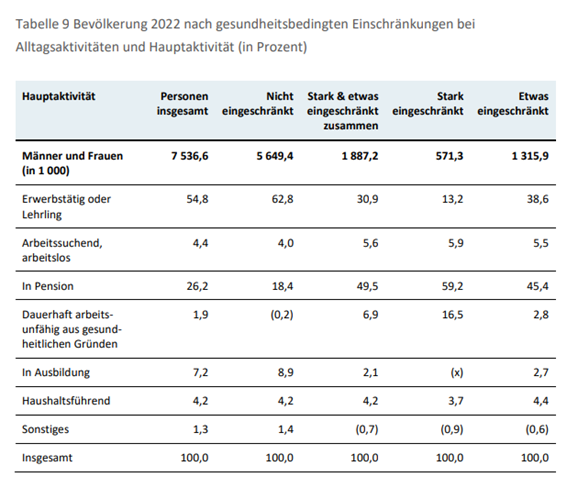
\includegraphics[scale=1]{pics/Statistik-Hauptaktivitaet.png}
    \caption{Statistik Hauptaktivitaet}
    \label{fig:statistik-2}
\end{figure}

(Quelle1, Quelle2)

\section{Interviews}
Im Rahmen eines Projekts bestand die Möglichkeit, einige Menschen kennenzulernen und 
mit diese Interviews über ihre Erfahrungen im Rollstuhl zu führen. Die Untersuchung zeigt, dass 
die zu bewältigende physische Herausforderung von emotionaler Stärke, dem Umgang mit der Umwelt 
sowie einem persönlichen Lebenswillen begleitet wurde, die sich auf unterschiedliche Weise äußerten. 
Die Gründe für die Pflegebedürftigkeit der Testpersonen waren heterogen. So waren die Betroffenen 
entweder dauerhaft oder vorübergehend auf einen Rollstuhl angewiesen. Ihre Geschichten demonstrieren 
die Diversität des Lebens mit einer Mobilitätseinschränkung und die Implikationen, die sich aus der 
Notwendigkeit ergeben, plötzlich oder von Geburt an auf Hilfe oder Hilfsmittel angewiesen 
zu sein.

\subsection{Zusammenfassung Interview 1}
Anna, 18 Jahre alt, erlitt vor vier Jahren einen schweren Unfall, in dessen Folge sie eine 
körperliche Beeinträchtigung erlitt, die für eine kurze Phase der Pflegebedürftigkeit in 
einem Rollstuhl erforderlich machte. Diese Wandelung vollzog sich in einem zeitlichen begrenzten, 
abrupten Ausmaß.

Nach dem Unfall wurde sie für die Dauer von einer Woche in ein Krankhaus gebracht. Sie sah sich 
mit der Herausforderung konfrontiert, sämtliche Alltagsaktivitäten neu zu erlenen. Hierzu zählten 
die eigenständige An- und Auskleidung sowie die Nutzung von Hilfsmitteln zur Körperpflege und die 
selbstständige Bedienung des Rollstuhls. Zunächst überwog eine ausgeprägte Verzweiflung. 
Allmählich manifestierte sich eine Veränderung. Es gelang ihr, sowohl eine physische als auch 
eine psychische Regeneration zu erfahren. Dennoch gestaltete sich der Übergang zurück in den 
Alltag als eine Abfolge kleiner, unerwarteter Schwierigkeiten. 

Nach dem Bruch ihrer Hüfte war Anna für die Dauer einer Woche auf einen Rollstuhl angewiesen für
eine kurze Zeit, jedoch stellte sie für sie eine völlig neue Erfahrung dar. Es wurde eine 
deutliche Verschlechterung der täglichen Routinen beobachtet, die sich in einfachen 
Verrichtungen wie dem Aufstehen am Morgen, dem Anziehen oder dem Duschen äußerte. Es oblag 
ihr, eine Vielzahl alltäglicher Abläufe neu zu erlernen oder dieses unter Zuhilfenahme von 
Hilfsmitteln zu bewältigen.

Der Schulbesuch stellte eine besondere Herausforderung dar. Das Gebäude entsprach nicht den 
Anforderungen der Barrierefreiheit, da es über keinen Aufzug verfügte, obwohl sich zahlreiche 
Unterrichtsräume in den oberen Stockwerken befanden. Die Bewältigung von Treppen stellt ein
Hindernis dar, die durch die physische und mentale Barriere der Überwindung charakterisiert ist. 
In viele Fällen war Improvisation unumgänglich. Die Schülerin wurde in andere 
Räumlichkeiten umgeleitet oder mit der Bearbeitung der Aufgaben zu Hause beauftragt. In der Folge 
verspürte sie eine Abkehr von der Klassengemeinschaft.

Die Zeit nach dem Unfall stellte sich zudem als eine physisch sowie psychisch belastenden Zeit 
heraus. Die plötzliche Notwendigkeit, auf die Unterstützung anderer angewiesen zu sein, 
beispielsweise beim Tragen der Schultasche, beim Öffnen von Türen oder beim Fortbewegen, wurde 
als ungewohnt und schmerzhaft empfunden. Die zuvor als selbstständig beschriebene Person sah 
sich plötzlich gezwungen, fortwährend um Hilfe zu ersuchen.

Besonders schwer wog dabei das Gefühl der Hilflosigkeit. Es 
ging einher mit der Angst, nie wieder vollständig zu genesen, und der Sorge, von anderen 
nur noch über die Verletzung definiert zu werden.

Obwohl sie den Rollstuhl nur temporär benötigte, führte diese Phase zu einer signifikanten 
Veränderung ihrer Perspektive auf zahlreiche Aspekte. Sie erlangte die Einsicht, dass sich das 
Leben mitunter rapide wandeln kann und dass es von großer Wichtigkeit ist, Geduld mit sich 
selbst zu bewahren.

\subsection{Zusammenfassung Interview 2}
Lukas, Alter 15, ist seit Mitte des Jahres 2024 auf einen Rollstuhl angewiesen, nachdem er 
infolge eines Unfalls für mehrere Monate immobil war. Die vorliegende Untersuchung widmet sich der
Thematik der Anpassung an eine neue körperliche Realität sowie den damit einhergehenden Veränderungen 
im alltäglichen Leben. Die Transition vom selbstständigen Gehen zur Nutzung eines Rollstuhls stellte 
eine einschneidende Erfahrung dar, die mit physischen und psychischen Herausforderungen einherging.

Der initiale Zustand des Alltags war durch eine signifikant ausgeprägte Fremdheit gekennzeichnet. 
Tätigkeiten, die zuvor als selbstverständlich erachtet wurden, wie das Überwinden von Stufen oder 
das selbstständige Bewegen über unebene Flächen, erforderten plötzlich fremde Hilfe. Die Abhängigkeit 
von anderen Personen wurde insbesondere in Bezug auf das Überwinden von Barrieren oder das Erreichen 
höhergelegener Orte als belastend empfunden. Im Zeitverlauf manifestierte sich eine zunehmende Routine. 
Lukas beschreibt, dass er sich in kurzer Zeit mit der Funktionsweise des Rollstuhls vertraut machte und 
die anfängliche Unsicherheit allmählich einer gewissen Selbstverständlichkeit wich.

Nichtsdestotrotz stellte die Mobilität eine Herausforderung dar. Er betont, dass Situationen ohne 
helfende Personen oft mit Anstrengung und Frustration verbunden waren. Wurde er von jemand anderem 
geschoben, so empfand er dies als ungewohnt und teilweise beunruhigend, da sich der Rollstuhl in
diesen Momenten instabiler und schneller anfühlte. Das Empfinden der Fremdbestimmung konstituierte 
eine mentale Hürde, die über die rein körperliche Einschränkung hinausging.

Besonders problematisch gestaltete sich die Situation im öffentlichen Verkehr. Obwohl Lukas in der 
Regel von einer Begleitperson unterstützt wurde, wiesen alltägliche Wege, etwa das Einsteigen in
Bus oder Zug, ein potenzielles Gefahrenpotential auf. Bereits geringfügige Unebenheiten, wie der 
Übergang von der Straße auf den Gehsteig, können als problematisch erachtet werden. Glücklicherweise 
blieb er von Stürzen verschont, war sich jedoch der ständigen Möglichkeit bewusst, dass solche 
Situationen leicht außer Kontrolle geraten können. Es liegen keine Erfahrungen mit elektrischen oder 
sportlichen Spezialrollstühlen vor. 

Die schulische Umgebung wurde von Lukas als barrierefrei beschrieben. Im Vergleich zu seiner früheren 
Schule, in der große Teile des Gebäudes nicht zugänglich waren, konnte er in seiner aktuellen 
Einrichtung fast alle Räume erreichen. Lediglich in Einzelfällen wurden Hindernisse festgestellt, 
die den Zugang erschwerten.

Seit Anfang 2025 ist Lukas wieder in der Lage, ohne Rollstuhl zu gehen. Die Phase der eingeschränkten
Mobilität hinterließ dennoch einen nachhaltigen Eindruck. Dies resultierte in einer vertieften 
Auseinandersetzung mit Themen wie Selbstständigkeit, Barrierefreiheit und gesellschaftlicher Inklusion. 
Obwohl er bislang keine Reisen ins Ausland unternommen hat, gab er an, dass er einen Aufenthalt in Wien 
absolviert hat. Dort habe er kaum Unterschiede zur Barrierefreiheit in Linz wahrgenommen.

Er äußert sich kritisch über den öffentlichen Verkehr. Insbesondere für Menschen, die vollständig auf 
den Rollstuhl angewiesen sind, ist der Einstieg in Züge oder Busse ohne fremde Hilfe nahezu unmöglich. 
In diesem Bereich wird ein erheblicher Bedarf an Verbesserungen identifiziert. Taxis und private Autos 
werden hingegen als die verlässlichsten und komfortabelsten Fortbewegungsmittel bezeichnet.

Zusammenfassend lässt sich festhalten, dass Lukas Erfahrung im Rollstuhl eine signifikante Veränderung 
seines Blicks auf den Alltag bewirkt hat. Es wurde ersichtlich, dass die physischen Grenzen urbaner 
Mobilität nicht die einzigen Faktoren sind, die in Bezug auf städtische Mobilität zu berücksichtigen 
sind. Darüber hinaus wurden auch die emotionalen Aspekte von Abhängigkeit, Unsicherheit und Anpassung 
evident. Trotz der temporären Natur dieser Einschränkung bleibt diese Zeit für ihn prägend, als Phase 
der Erkenntnis, wie fragil Selbstständigkeit sein kann und wie wesentlich Empathie und Barrierefreiheit 
im gesellschaftlichen Zusammenleben sind.


\subsection{Zusammenfassung Interview 3}
Tom, 32 Jahre alt, ist seitdem er geboren ist infolge einer körperlichen Beeinträchtigung, die eine 
dauerhafte Rollstuhlabhängigkeit bedingt, behindert. Sein Alltag ist geprägt von einer Kombination aus 
Routine, Anpassung und der permanenten Auseinandersetzung mit einer Umwelt, die nicht immer barrierefrei 
gestaltet ist. Die vorliegende Darstellung befasst sich mit den physischen und psychischen 
Herausforderungen, die das Leben im Rollstuhl mit sich bringt, sowie mit den gesellschaftlichen und 
infrastrukturellen Bedingungen, die seinen Alltag maßgeblich beeinflussen.

Das Fortbewegen auf unebenem Untergrund, etwa auf Kopfsteinpflaster oder auf schmalen, uneben Wegen, 
stellt für Tom eine erhebliche Herausforderung dar. Das Befahren solcher Flächen erfordert ein hohes Maß 
an Konzentration und Kraft. Er beschreibt das subjektive Empfinden als mühsam und unangenehm, da jede 
Bewegung abgebremst und erschüttert wird. In vielen Fällen ist eine nur sehr langsame Progredienz zu 
beobachten. Zudem besteht eine konstante Angst, das Gleichgewicht zu verlieren oder in einer Vertiefung 
des Geländes stecken zu bleiben. In solchen Momenten ist er gezwungen, seine Aufmerksamkeit vollständig 
auf die Bewegung zu richten, wodurch der eigentliche Spaziergang oder Ausflug an Leichtigkeit einbüßt.

Stufen, Bordsteinkanten und größere Höhenunterschiede stellen dabei die größten Herausforderungen dar. 
Während geringe Schwellen mit einer gewissen Dynamik überwunden werden können, stellen Treppen oder 
Bodenlücken eine unüberwindbare Barriere dar. In solchen Fällen ist Tom auf Unterstützung angewiesen, 
die zumeist durch Familienmitglieder oder Freunde erfolgt, die ihn begleiten. Die Analyse der vorliegenden 
Daten ergibt, dass Alleinreisen nur selten praktiziert werden können. Tom lebt mit seiner Familie, die 
ihn in den meisten Situationen unterstützt. Dennoch empfindet er es als belastend, nicht immer autonome 
Handlungsfähigkeit zu haben. Das Ersuchen um Unterstützung wird von ihm mit einem Gefühl der Abhängigkeit 
assoziiert, welches er nur schwer akzeptieren kann.

Tom misst der Gestaltung öffentlicher Räume eine besondere Bedeutung bei. Er betont, dass Rampen, 
barrierefreie Übergänge und glatte Wege die Lebensqualität von Rollstuhlnutzern erheblich steigern 
können. Als besonders positiv hebt er seine Erfahrungen an einem Strand hervor, an dem spezielle Wege 
bis hin zum Meer angelegt waren. Diese Fähigkeit ermöglichte es den Menschen, sich selbständig 
fortzubewegen und das Meer aus eigener Kraft zu erreichen. Dies vermittelte ihnen ein Gefühl von 
Freiheit und Selbstbestimmung.

Darüber hinaus verweist Tom auf die mangelnde Infrastruktur für Rollstuhlfahrer, etwa fehlende 
Parkplätze, zu enge Wege oder unzureichend angepasste Hotelzimmer. Insbesondere das Reisen stellt 
für ihn und seine Familie eine finanzielle und organisatorische Herausforderung dar. Hotels, die 
über rollstuhlgerechte Badezimmer und barrierefreie Zugänge verfügen, sind häufig mit höheren Kosten 
verbunden und in vielen Regionen nur begrenzt verfügbar.

Tom beobachtet zudem kulturelle Unterschiede im Umgang mit Menschen mit Behinderung. In einigen 
Kulturkreisen werden freundliche und hilfsbereite Absichten zwar positiv bewertet, jedoch zeigt Tom 
eine gewisse Skepsis gegenüber dieser, als übertrieben empfundenen Verhaltensweisen, die er mit Mitleid 
verbindet. Er bevorzugt einen natürlichen und respektvollen Umgang, der seine Beeinträchtigung nicht als 
ausschließlich bestimmenden Faktor betrachtet.

Mit zunehmendem Alter bemerkt auch seine Mutter, die ihn oft schiebt, dass die körperliche Belastung zunimmt. 
Das gemeinsame Unterwegssein wird zunehmend als belastend empfunden, sowohl von der Frau als auch von 
Tom empfunden. Dies veranschaulicht, dass Barrierefreiheit nicht nur den Betroffenen selbst, sondern auch 
deren Angehörigen zugutekommt.

Des Weiteren beschreibt Tom das unangenehme Gefühl, welches sich einstellt, wenn er, etwa während des 
Umsteigens aus dem Rollstuhl, von anderen beobachtet wird. In diesen Momenten verspürt er ein Gefühl 
der Exposition, Verletzlichkeit und Bewertung. Die Familie des Betroffenen zeigt eine hohe Aufmerksamkeit 
für die Wahl von Orten, die über Rampen verfügen, um das Eintreten solcher Situationen zu vermeiden.

Es lässt sich festhalten, dass der Alltag des Probanden von einem stetigen Wechsel zwischen 
Selbstständigkeit und Abhängigkeit geprägt ist. Seine Erfahrungen zeigen, dass die Gestaltung 
öffentlicher Räume, Straßen und Gebäude einen entscheidenden Einfluss darauf hat, in welchem Maß 
Menschen mit Mobilitätseinschränkungen am gesellschaftlichen Leben teilhaben können. Trotz zahlreicher 
Herausforderungen zeigt Tom eine bemerkenswerte Gelassenheit. Er erkennt in jeder barrierefreien Rampe, 
in jedem angepassten Raum einen Aspekt des gesellschaftlichen Fortschritts und ein Indiz dafür, dass 
Inklusion nicht nur ein theoretisches Ideal, sondern eine alltägliche Notwendigkeit ist.

(Quelle 3, 4, 5)

\begin{spacing}{1}
\chapter{Umfeldanalyse}
\end{spacing}
\setauthor{Elisa Kaltenberger}

\section{Gesellschaftliches Umfeld}
\setauthor{Elisa Kaltenberger}
Ein großer Teil der Bevölkerung nimmt alltägliche körperliche Aktivitäten als selbstverständlich wahr. Für Menschen mit körperlichen Einschränkungen ist diese Selbstverständlichkeit jedoch häufig nicht oder nur eingeschränkt gegeben. Barrieren, die für viele kaum wahrnehmbar sind, können für Betroffene nicht bewältigt werden. Dazu zählen unter anderem nicht abgesenkte Bordsteinkanten, unebene Pflastersteine oder zu niedrig platzierte Bankautomaten mit zu hohem Sichtschutz.

Die eingeschränkte Zugänglichkeit zu Infrastruktur und Dienstleistungen wirkt sich nicht ausschließlich auf  die Mobilität aus, sondern betrifft in hohem Maß die gleichberechtigte gesellschaftliche Teilhabe.  Selbstbestimmung, soziale Integration und berufliche Möglichkeiten hängen wesentlich davon ab, wie  barrierefrei öffentliche und private Räume gestaltet sind.

Mit steigender Lebenserwartung nimmt auch die Anzahl jener Personen zu, die temporär oder dauerhaft auf  Unterstützung angewiesen sind. Barrierefreiheit ist daher kein Randthema, sondern betrifft einen signifikanten Teil der Bevölkerung, siehe Abb. \ref{fig:lebensqualiteat}.

\section{Erfahrungsberichte aus Interviews}
\setauthor{Elisa Kaltenberger}
Die Berichte zeigen, dass Mobilitätseinschränkungen sowohl temporär als auch dauerhaft auftreten können. 
Besonders auffallend ist dabei nicht nur die physische Herausforderung, sondern auch die psychische. 
Gefühle wie Abhängigkeit, Unsicherheit oder Hilflosigkeit treten häufig auf, insbesondere wenn alltägliche 
Handlungen plötzlich nicht mehr selbstständig durchgeführt werden können.

Häufige Probleme die in den Interviews genannt wurden, sind:
\begin{itemize}
    \item Schwierigkeiten beim Überwinden von Stufen und Bordsteinkanten
    \item Probleme im öffentlichen Verkehr
    \item Unangenehmes fahren auf unebenem Untergrund (z.B. Pflastersteine)
    \item Abhängigkeit von fremder Hilfe
\end{itemize}

Gleichzeitig wurde deutlich, dass barrierefreie Maßnahmen wie Rampen, abgesenkte Übergänge oder gut 
zugängliche öffentliche Räume erheblich zur Selbstständigkeit und Lebensqualität beitragen können.

\section{Zielgruppe des Projekts}
\setauthor{Elisa Kaltenberger}

Die Zielgruppe des Projekts umfasst unterschiedliche Personengruppen, die direkt oder indirekt mit dem Thema 
Barrierefreiheit in Berührung kommen. 

Dazu zählen insbesondere Menschen, die in der Stadtplanung oder 
Architektur tätig sind, da sie maßgeblich an der Gestaltung öffentlicher Räume beteiligt sind und durch ein 
vertieftes Verständnis der Problematik barrierefreie Strukturen gezielter umsetzen können und somit mehr 
gleichberechtigte Teilhabe ermöglichen können.

Ebenso richtet sich die Simulation an Personen, die beruflich oder ehrenamtlich im Bereich der 
Barrierefreiheit arbeiten. Für diese bietet das Projekt eine zusätzliche Möglichkeit die Perspektiven 
anschaulich zu vermitteln und Sensibilisierungsarbeit praxisnah zu unterstützen.

Darüber hinaus gehören Angehörige von Menschen mit Mobilitätseinschränkungen zur Zielgruppe. Sie können 
durch die Simulation einen besseren Einblick in die alltäglichen Herausforderungen erhalten und dadurch 
mehr Verständnis für die Lebensrealität ihrer Familienmitglieder entwickeln und somit die Unterstützung 
gezielter gestalten und sich auf die Bedürfnisse der Betroffenen besser einstellen.

Eine weitere Zielgruppe sind alle, die nach einem Unfall kurz davor stehen, selbst auf einen Rollstuhl 
angewiesen zu sein. Für diese Personen bietet die Simulation die Möglichkeit, sich bereits vorab mit der 
neuen Lebenssituation auseinanderzusetzen und sich auf die Herausforderungen einzustellen. Dadurch kann 
die Simulation nicht nur zur Sensibilisierung beitragen, sondern auch als unterstützendes Werkzeug für die 
Vorbereitung auf die neue Lebensrealität dienen.



\begin{spacing}{1}
\chapter{Ideenfindung}\label{chapter:ideenfindung}
\end{spacing}
\setauthor{Elisa Kaltenberger}

Die Projektidee entstand aus eigenem Interesse und der grundlegenden Fragestellung, wie Barrierefreiheit im Alltag tatsächlich erlebt wird, insbesondere aus der Perspektive von Rollstuhlfahrenden. Im schulischen und gesellschaftlichen Kontext wird Barrierefreiheit häufig theoretisch behandelt, jedoch selten praktisch erfahrbar gemacht.

Ein weiterer Ausgangspunkt war das Interesse an immersiven Technologien wie Virtual Reality. VR bietet die Möglichkeit, Perspektiven realitätsnah zu simulieren und Nutzer*innen unmittelbar in eine andere Lebenssituation zu versetzen. Dadurch entstand die zentrale Leitfrage:

\textbf{Wie kann man typische Hindernisse für Rollstuhlfahrende so darstellen, dass Außenstehende 
diese nicht nur sehen, sondern selbst erleben?}

Im nächsten Schritt wurden konkrete Alltagssituationen analysiert. Durch Recherche und Gespräche 
wurde deutlich, dass insbesondere folgende Hindernisse immer wieder problematisch sind:

\begin{itemize}
    \item zu hoch angebrachte Bankautomaten
    \item nicht abgesenkte oder zu hohe Bordsteinkanten
    \item unebene Pflastersteine
\end{itemize}

Diese Beobachtungen führten zur Entscheidung, eine virtuelle Stadtumgebung zu entwickeln, in der genau 
diese Herausforderungen gezielt eingebaut werden.

Im Verlauf der Projektentwicklung wurde deutlich, dass eine rein visuelle VR-Simulation zwar die 
Perspektive verändern kann, jedoch das körperliche Empfinden nur eingeschränkt vermittelt. Aus diesem Grund 
entstand die weiterführende Idee, zusätzlich einen Hardware-Simulator zu entwickeln.

Ziel dieses Simulators war es, die Bewegungen aus der realen Welt präzise in die virtuelle Umgebung zu 
übertragen und die Bewegungen der VR-Welt physisch spürbar zu machen. Dadurch sollte nicht nur es nicht nur
visuell dargestellt werden, sondern auch ein mechanisches Feedback erzeugt werden.

Der entwickelte Aufbau ermöglicht es, reale Bewegungen, beispielsweise das Überfahren einer Kante oder einer 
unebenen Oberfläche, direkt an die Hardware-Simulation weiterzugeben. Gleichzeitig werden Bewegungsimpulse aus der 
Simulation mechanisch umgesetzt, sodass Nutzer*innen Höhenunterschiede oder Neigungen tatsächlich wahrnehmen 
können.

\begin{spacing}{1}
\chapter{Handbuch}\label{chapter:handbuch}
\end{spacing}

Dieses Handbuch beschreibt die Installation, den Aufbau sowie die Bedienung der im Rahmen der Diplomarbeit 
entwickelten VR-Simulation. Die Anwendung wurde mit Unity entwickelt und ermöglicht die 
Perspektive von Rollstuhlfahrenden in einer virtuellen Stadtumgebung einzunehmen.

Ziel der Simulation ist es, typische Hindernisse wie Bankautomaten, Bordsteinkanten und Pflastersteine 
realitätsnah erfahrbar zu machen und deren Auswirkungen auf die Mobilität nachvollziehbar darzustellen.

\section{VR-Welt}
\setauthor{Elisa Kaltenberger}
Zuerst wird Unity installiert und das Projekt geklont. Anschließend wird die entsprechende Szene geöffnet. Falls gewünscht, kann eine VR-Brille angeschlossen und die Szene gestartet werden. Weitere Einstellungen müssen nicht vorgenommen werden.

\subsection{Voraussetzungen}
\setauthor{Elisa Kaltenberger}
Für die Nutzung der Simulation werden folgende Komponenten benötigt:
\begin{itemize}
    \item Laptop oder PC mit installierter Unity-Version (passend zur Projektdatei)
    \item Optional: VR-Headset (z. B. Meta Quest 2 oder vergleichbares Gerät)
    \item Installierte Meta Quest Link-Software bei Verwendung einer Meta-Brille
    \item USB-C-Kabel zur Verbindung zwischen Headset und Computer
\end{itemize}

\subsection{Installation}
\setauthor{Elisa Kaltenberger}
\begin{itemize}
    \item Unity installieren (falls noch nicht vorhanden)
    \item Projektdatei klonen oder herunterladen
    \item Projekt über den Unity Hub öffnen
    \item Die Hauptszene im Projektordner auswählen und öffnen
    \item Optional: VR-Brille anschließen
    \item Auf „Play-Button“ klicken => die Simulation startet
\end{itemize}


\subsection{Ohne VR-Brille}
\setauthor{Elisa Kaltenberger}
Die Simulation kann auch ohne Headset direkt am Bildschirm getestet werden. Die Steuerun erfolgt über 
WSAD-Tasten und Pfeiltasten für die Bewegung und die Maus für die Blickrichtung. Es ist jedoch zu beachten, 
dass die Erfahrung ohne VR-Brille eingeschränkt ist, da die Immersion und das räumliche Bewusstsein reduziert 
sind.

\subsection{Mit VR-Brille}
\setauthor{Elisa Kaltenberger}
Für das vollständige immersive Erlebnis wird die Nutzung mit VR-Headset empfohlen.

\begin{itemize}
    \item Meta Quest Link starten
    \item VR-Brille per Kabel mit dem Laptop verbinden
    \item Warten, bis das Headset vom System erkannt wurde (dies kann einige Minuten dauern)
    \item Szene in Unity starten
\end{itemize}

Steuerung in VR:
\begin{itemize}
    \item Bewegung durch Neigen und Ausrichten der Controller in die gewünschte Richtung
    \item Kopfbewegungen steuern die Blickrichtung
\end{itemize}




\begin{spacing}{1}
\chapter{VR-Welt}\label{chapter:vr-world}
\end{spacing}
\section{Programmierumgebung finden}
\setauthor{Elisa Kaltenberger}

Für die vorliegende Diplomarbeit wurde die Unity Engine gegenüber der Unreal Engine aus mehreren, 
auf das Projekt zugeschnittenen Gründen ausgewählt. Die Entwicklung einer 3D-VR-Simulation erforderte 
eine sorgfältige Abwägung, wobei Unity insgesamt die bessere Eignung aufwies.
(Quelle1, Quelle2)

Der entscheidende Faktor war die gewohnte Programmierbasis. Da die schulische Ausbildung ausschließlich 
auf Java ausgerichtet war, bot Unity mit der Programmiersprache C-Sharp einen idealen und höchst effizienten 
Übergang. Die Ähnlichkeit der Sprachen in Syntax und objektorientierten Konzepten ermöglichte eine 
unmittelbare Übertragung des bestehenden Wissens auf die Engine-Programmierung. Dadurch war es möglich, 
den Fokus von Beginn an auf die spezifischen Herausforderungen der VR-Programmierung zu legen. Zu diesen 
Herausforderungen zählen beispielsweise Interaktion, Bewegung und die Optimierung der Performance für VR. 
Die Verwendung der Unreal Engine, die eine komplexere C++-Sprache sowie ein völlig anderes Blueprint-System 
erfordert hätte, hätte zu einem erheblichen Mehraufwand an Lernzeit geführt und somit wertvolle Zeit für die 
inhaltliche Entwicklung der Simulation in Anspruch genommen.
(Quelle1, Quelle3)

Zweitens ist Unity im Bereich VR/XR besonders gut aufgestellt und zugänglich. Über das XR Interaction Toolkit 
und die OpenXR-Unterstützung werden von Unity standardisierte und gut dokumentierte Frameworks speziell für die 
VR-Entwicklung angeboten. Diese Tools abstrahieren plattformspezifische Schwierigkeiten und ermöglichen einen 
effizienten Einstieg in die Entwicklung von Interaktionen für VR-Controller. Obwohl Unreal Engine ebenfalls 
über ausgeprägte VR-Fähigkeiten verfügt, wird der Einstieg in die VR-Interaktionsprogrammierung mit Unity 
aufgrund der hochwertigen, offiziellen Plugins oft als direkter und schulprojektfreundlicher empfunden.
(Quelle1, Quelle2, Quelle3)

Die Performance-Charakteristik wurde dahingehend modifiziert, dass eine bessere Passung zum Projekt erzielt 
wurde. Für eine stabile VR-Simulation ist eine hohe und konstante Framerate (FPS) von entscheidender Bedeutung, 
um das Auftreten von Motion Sickness zu vermeiden. Unity-Projekte werden als vergleichsweise ressourcenschonend 
und gut optimier- sowie kontrollierbar angesehen, was für den überschaubaren Umfang einer schulischen Simulation 
vorteilhaft war. Obwohl die Unreal Engine häufig eine beeindruckendere Grafik erzeugt, weist sie in zahlreichen 
Szenarien einen höheren "Basis-Overhead" auf und erfordert eine leistungsstärkere Hardware. Im Rahmen eines 
exemplarischen Simulationsprojekts, das sich durch eine starke Fokussierung auf die inhaltliche Interaktion 
auszeichnete, wurde Unity als die Lösung identifiziert, die ein optimales Verhältnis zwischen visueller Qualität 
und garantierter Leistung der verfügbaren Hardware aufwies. Dies steht im Gegensatz zu fotorealistischen 
Visualisierungen, die bei diesem Projekt nicht im Vordergrund standen.
(Quell1, Quelle2)

\section{Welt einrichten}
\subsection{Überlegung der Hindernisse}
Zunächst wurden die signifikanten Hindernisse für Rollstuhlfahrende identifiziert und einer Analyse unterzogen. 
Auf dieser Grundlage wurde anschließend die VR-Welt gestaltet, um ein möglichst realistisches und zugleich 
bestmögliches Ergebnis zu erzielen.

Für Menschen mit Mobilitätseinschränkungen kann die Nutzung eines Bankautomaten eine Herausforderung darstellen. 
In einer signifikanten Anzahl von Fällen sind die Automaten zu hoch angebracht, was dazu führt, dass sowohl der 
Bildschirm als auch das Tastenfeld nur mit einem hohen Aufwand erreicht werden können. In vielen Fällen ist die 
zur Verfügung stehende Bewegungsfläche vor dem Automaten unzureichend. Ein zusätzliches Problem stellt der 
Sichtschutz dar, da die seitlichen Schutzblenden oder Abdeckungen in der Regel für stehende Personen konzipiert sind.

Eine Bordsteinkante stellt für Rollstuhlfahrer*innen im Alltag eine signifikante Barriere dar. Die Höhe der 
Bordsteine hat einen signifikanten Einfluss auf die Fähigkeit der Verkehrsteilnehmer, die Straße selbstständig zu 
überqueren. Selbst geringfügige Höhenunterschiede können eine Gefahr darstellen, da die Räder im Rollstuhl hängen 
bleiben oder das Gefährt umkippen kann. Abgesenkte Bordsteine werden häufig als unzureichend gestaltet wahrgenommen 
oder deren Nutzung wird durch parkende Autos, Fahrräder oder Baustellen erschwert. Bei Niederschlag kommt es zu 
einer Wasseransammlung, was das Überfahren zusätzlich erschwert.

Des Weiteren ist festzustellen, dass Pflastersteine problematisch sind. Die unebene Oberfläche des Produkts 
führt zu einer signifikanten Erschütterung, die sich negativ auf die körperliche Verfassung auswirken kann. 
Es wurde beobachtet, dass insbesondere die kleinen Vorderräder des untersuchten Objekts in Fugen oder abgesackten 
Steinen hängen bleiben können. Bei Nässe oder Glätte können Pflastersteine eine erhöhte Rutschgefahr aufweisen, 
was das Unfallrisiko signifikant erhöhen kann. Zudem ist ein deutlich höherer Kraftaufwand erforderlich, um auf 
diesen Wegen zu reisen, was die Autonomie der Fortbewegung erheblich einschränkt.

\subsection{Erster Prototyp}
Der erste Prototyp der VR-Welt wurde in Unity erstellt, um die zuvor identifizierten Hindernisse für 
Rollstuhlfahrende zu simulieren. Dabei wurden verschiedene Umgebungen modelliert, die typische Herausforderungen 
im Alltag darstellen, wie z.B. Bankautomaten, Bordsteinkanten und Pflastersteine.

In der ersten konkreten Umsetzungsphase des Projekts wurde ein strategischer Fokus auf Funktionalität und 
Nutzerperspektive gelegt. Hierzu wurde bewusst auf den Import komplexer, fertiger 3D-Assets verzichtet. 
Unter „Assets“ versteht man in diesem Kontext vollständig texturierte Modelle wie Gebäude, Autos oder 
detaillierte Oberflächenmaterialien, die üblicherweise für die visuelle Vollendung einer virtuellen 
Umgebung genutzt werden.

Stattdessen wurde eine minimalistische, abstrakte Testumgebung erstellt, die auch als Whitebox- oder 
Greybox-Prototyp bezeichnet wird. Die vorliegende Struktur besteht ausschließlich aus einfachen 
geometrischen Grundkörpern, die direkt innerhalb der Unity Engine erzeugt und arrangiert wurden. 
Die gesamte Szene wurde folglich in einer reduzierten, häufig einfarbigen oder grob gerasterten 
Darstellung präsentiert.
(Quelle ITP Buch)

Das primäre und ausschließliche Ziel dieser Phase war die funktionale Validierung der zentralen Hindernisse 
ausschließlich aus der spezifischen Perspektive eines Rollstuhlfahrers. Es ging nicht um realistische 
Darstellung, sondern um die Beantwortung essenzieller technischer und konzeptioneller Fragen: Werden die 
Hindernisse aus der festgelegten Sitzhöhe korrekt und eindeutig wahrgenommen? Funktioniert die physikalische 
Kollisionserkennung an Bordsteinen und Kanten wie intendiert? Löst die Platzierung eines simulierten 
Bankautomaten das gewünschte Interaktionsproblem (Unerreichbarkeit, eingeschränkte Sicht) aus? Wie fühlt 
sich die Bewegung über ein Feld unebener Pflastersteine in der reinen Gameplay-Logik an? 

\begin{figure}
    \centering
    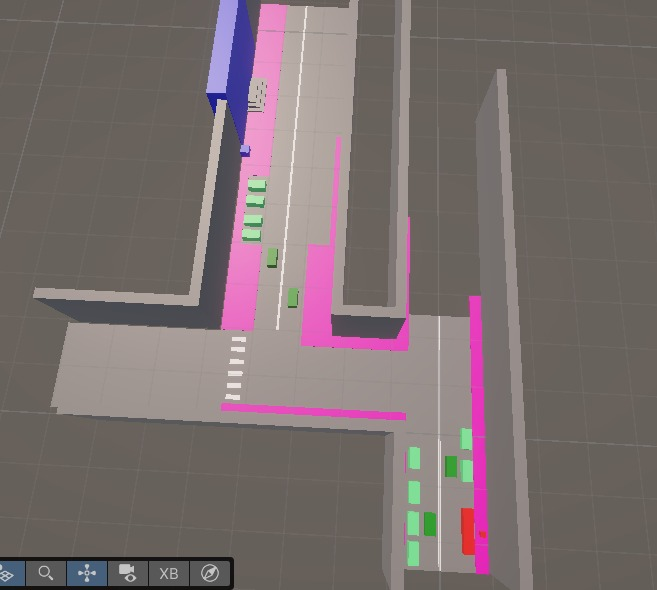
\includegraphics[scale=0.5]{pics/prototyp-welt.jpg}
    \caption{Prototyp der VR-Welt mit Hindernissen für Rollstuhlfahrende}
    \label{fig:vr-world:prototyp}
\end{figure}

\subsection{Welt gestalten}
Nach erfolgreicher Einrichtung der Testumgebung wurde ein umfangreiches Asset-Paket einer realen Stadt 
ausgewählt und heruntergeladen. Im Anschluss daran wurden die einzelnen Gebäude manuell aus dem Paket 
extrahiert, separat aufbereitet und in die virtuelle Realität integriert. Um die Szenerie lebendiger 
und authentischer wirken zu lassen, wurden zusätzliche Elemente wie detailreiche Gehsteige, verschiedene 
Fahrzeugmodelle sowie ein vollständiges Straßennetz systematisch hinzugefügt.

Die Modellierung, Texturierung und Integration der weiteren ästhetischen Komponenten, welche nicht durch 
das Asset-Paket abgedeckt waren, erfolgte individuell. Im Anschluss wurden diese in die virtuelle 
Umgebung implementiert. Der kreative und technische Prozess, der zur Schaffung einer immersiven, 
kohärenten und visuell ansprechenden VR-Landschaft führte, ist als erfolgreich zu betrachten.

\begin{figure}
    \centering
    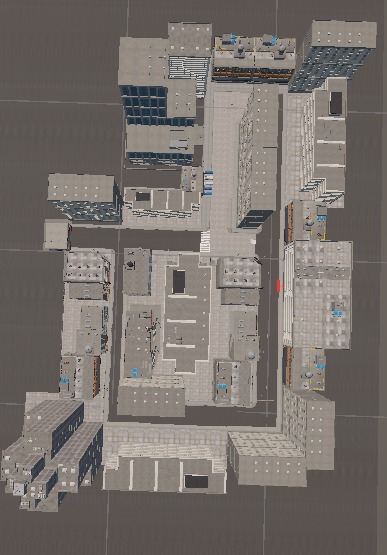
\includegraphics[scale=0.7]{pics/umgesetzte-welt.jpg}
    \caption{Umgesetzte VR-Welt mit Hindernissen für Rollstuhlfahrende}
    \label{fig:vr-world:umgesetzte-welt}
\end{figure}




\begin{spacing}{1}
\chapter{Bewegungen im Virtuellen Raum}\label{chapter:cyber_sickness}
\end{spacing}
Der Begriff Virtual Reality, im Folgenden als VR bezeichnet, beschreibt die Darstellung und simultane Wahrnehmung einer echt erscheinenden Realität und ihren physikalischen Eigenschaften in einer in Echtzeit computergenerierten, interaktiven virtuellen Umgebung.

Die Beliebtheit von VR-Technologie hat in jüngerer Vergangenheit einen deutlichen Aufschwung erlebt, der insbesondere auf die Markteinführung einer Reihe kostengünstiger VR-Headsets zurückzuführen ist. Hierzu zählen Oculus, HTC Vive, PlayStation VR und Google Cardboard. Das bereits seit geraumer Zeit bestehende Problem der Cyberkrankheit konnte bislang nicht vollständig gelöst werden und wird aller Voraussicht nach ein signifikantes Hindernis für die flächendeckende Einführung von VR darstellen.

\section{Definition Motion Sickness, Cybersickness, VRISE}
\setauthor{Linnea Schönbauer}
Bei zahlreichen Menschen, sind bei der Nutzung eines Fahrzeugs der Stärke nach
variierende Krankheitssymptome zu beobachten. Zu den möglichen Nebenwirkungen zählen, beispielsweise, Übelkeit, Kopfschmerzen, Schwindel und weitere Beschwerden, die umgangssprachlich als Reise- oder Bewegungskrankheit bzw. vor allem im internationalen Raum als Motion Sickness bezeichnet werden.

Cybersickness, auch Virtual Reality Induced Sickness Effects (VRISE), genannt, weist laut Studien (QUELLE1) starke Ähnlichkeiten zu Motion Sickness auf. Obwohl die Situationen, die sie verursachen, leicht differieren, können die zugrunde liegenden Mechanismen auf die gleiche Weise erklärt werden. Cybersickness ist ein Phänomen, das mit physischen und psychischen Beeinträchtigungen einhergeht. Es manifestiert sich nach dem Experimentieren mit VR-Anwendungen und kann stundenlang anhalten. Die Diskrepanzen zwischen den wahrgenommenen Bewegungen in der realen und der virtuellen Welt sind dabei von zentraler Bedeutung.

\section{Biologische Ursachen von Cybersickness}
\setauthor{Linnea Schönbauer}
Im vorherigen Punkt wird bereits klargestellt, dass die Symptome der Cybersickness das Befinden der Nutzer:innen einer VR-Software immens beeinflussen. Deshalb muss ein Weg gefunden werden, um diese Beschwerden möglichst zu reduzieren.

Um die Faktoren zu bestimmen, die das Auftreten von Symptomen der VR-Krankheit bedingen, ist zunächst eine klare Definition des Konzepts der Eigenbewegung und dessen zwei Hauptkomponenten erforderlich.

\subsection{Das Gleichgewichtssystem}
\begin{figure}[htbp]
    \centering
    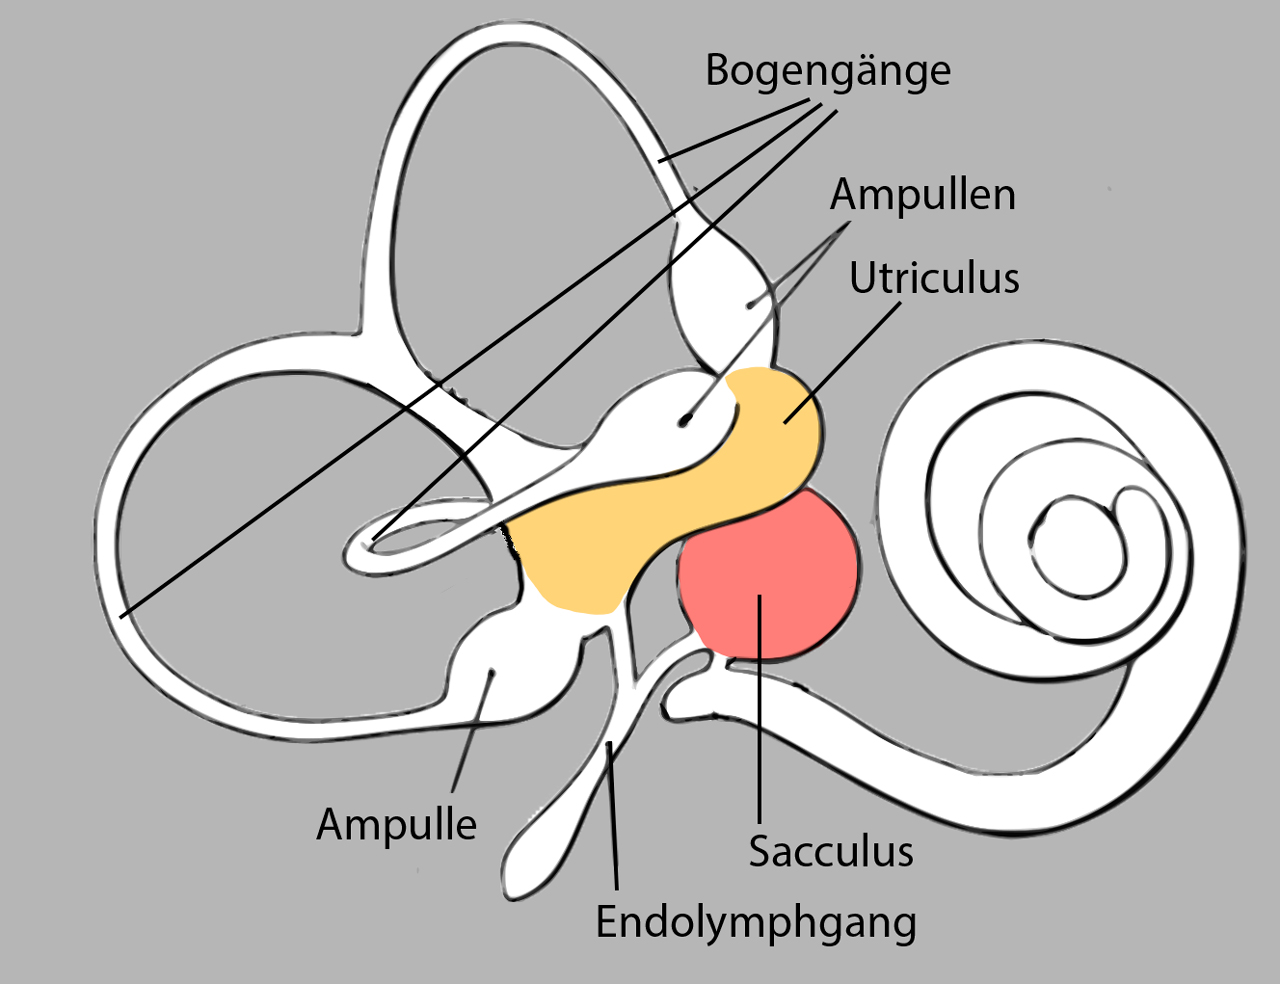
\includegraphics[scale=0.2]{pics/vestibular-system.jpg}
    \caption{Vestibuläres System}
    \label{fig:cybersickness:vestibular-system}
\end{figure}

Das Gleichgewichtssystem, auch vestibuläres System genannte, befindet sich im Innenohr und ist für die Wahrnehmung von Bewegung  und Orientierung im Raum verantwortlich. Es besteht aus drei Bogengängen, die Drehbewegungen des Kopfes erfassen, sowie dem Utriculus und dem Sacculus, die lineare Beschleunigungen und die Lage zur Schwerkraft registrieren. Gemeinsam liefern sie dem Gehirn Informationen darüber, wie sich der Kopf - und damit der Körper - im Raum bewegt.

\subsection{Das Visuelle System}
Dieses eben erwähnte Gleichgewichtssystem arbeitet eng mit dem visuellen System zusammen. Während die Augen visuelle Eindrücke von Bewegung liefern, sorgt das vestibuläre System dafür dass die tatsächlichen Bewegungen des Kopfes erkannt und ausgeglichen werden. Diese geschieht unter anderem durch den sogenannten vestibulo-okulären Reflex, der die Augen stabilisiert, wenn sich der Kopf bewegt. (QUELLE2)

Stimmen die Signale von Auge und Gleichgewichtssystem jedoch nicht überein, kann eine Sinnestäuschung entstehen. So kann man sich beispielsweise auch ohne tatsächliche Bewegung bewegt fühlen, wenn sich das Sichtfeld verändert. Dieser Effekt wird als Vection bezeichnet. Solche Wahrnehmungskonflikte zwischen Augen und Gleichgewichtssinn sind eine zentrale Ursache für Cybersickness, also die Übelkeit oder Desorientierung, die in virtuellen Umgebungen auftreten kann.

\section{Ursachen für Cybersickness in der virtuellen Realität}
Nachdem geklärt wurde, auf welche zwei wichtigen biologischen Faktoren die Cybersickness in der echten Welt zurückzuführen ist, muss nun untersucht werden, warum die Symptome beim Verwenden einer VR-Software auftreten.
Die Ursachen für Cybersickness werden unter anderem durch die \emph{Sensory Conflict Theory} (Theorie des sensorischen Konflikts), die \emph{Poison Theory} (Vergiftungshypothese) und die \emph{Postural Instability Theory} (Theorie der posturalen Instabilität) beschrieben (QUELLE4).

\subsection{Sensory Conflict Theory}
Die Sensory-Conflict-Theorie gilt als die älteste und am weitesten akzeptierte Erklärung für Cybersickness.(QUELLE5QUELLE2) Demnach wird Cybersickness durch Diskrepanzen zwischen den für die Wahrnehmung von Bewegung und Orientierung zuständigen Sinnen ausgelöst. Besonders relevant ist dabei der Konflikt zwischen dem visuellen und dem vestibulären System. (SIEHE KAPITEL DAS GLEICHGEWICHTSSYSTEM) Tritt eine Situation auf, in der das visuelle System signalisiert, das vestibuläre System jedoch keine entsprechende physische Bewegung registriert, entsteht ein wahrnehmungsbasierter Konflikt, den der Körper nicht korrekt verarbeiten kann.

Ein typisches Beispiel hierfür ist ein virtueller Fahrsimulator: Während der Nutzer visuell die Bewegung auf der Straße und das Vorbeiziehen von Gebäuden wahrnimmt, bleibt sein Körper statisch. Da das vestibuläre System keine Informationen über Beschleunigung oder Drehungen liefert, entsteht ein Mismatch der Sinneseindrücke, das Cybersickness hervorrufen kann. Diese Theorie wird durch zahlreiche Studien unterstützt.(QUELLE6QUELLE7) Sie betont die zentrale Rolle des visuell-vestibulären Konflikts, weist jedoch auch Einschränkungen auf: So kann sie beispielsweise nicht zuverlässig vorhersagen, wer unter Cybersickness leidet oder wie stark die Symptome ausfallen. Auch erklärt sie nicht vollständig, warum manche Personen empfindliche reagieren als andere. 

\subsection{Poison Theory}
Die Poison-Theorie versucht, die Entstehung von Cybersickness aus evolutionärer Sicht zu erklären.(QUELLE8) Demnach dienen Übelkeit und Erbrechen ursprünglich als Schutzmechanismus, um den Körper vor aufgenommenen Giften zu warnen und diese aus dem Magen zu entfernen. Bei Cybersickness kann die inadäquate Stimulation der visuellen und vestibulären Systeme dazu führen, dass der Körper die Sinneseindrücke falsch interpretiert und glaubt, eine giftige Substanz aufgenommen zu haben. Dadurch treten Symptome wie Übelkeit auf.(QUELLE2QUELLE5)

Einige Studien(QUELLE9QUELLE10) unterstützen diese Hypothese und zeigen, dass die Symptome in sehr spezifischen Situationen reduziert werden können. Dennoch ist die Theorie umstritten, da sie kaum Vorhersagekraft hat und nicht erklärt, warum manche Personen bei identischen Reizen in virtuellen Umgebungen Cybersickness entwickeln, andere jedoch nicht. Zudem erscheint der zeitliche Ablauf evolutionär problematisch, da Toxine zu lange brauchen würden, um die vestibulären Mechanismen auszulösen, sodass Erbrechen nicht effektiv wäre. Daher ist die Validität der Theorie bislang schwer nachzuweise. Sie wird eher als interessante Hypothese betrachtet, die bei der Gestaltung von VR-Erfahrungen vorsichtig berücksichtigt werden sollte.

\subsection{Postural Instability Theory}
Die von Ricco und Stoffregen entwickelte Postural-Instability-Theorie besagt, dass Cybersickness durch anhaltende Haltungsinstabilität entstehen. Der Mensch strebt danach, seine posturale Stabilität aufrechtzuerhalten, das heißt, einen Zustand zu erreichen, in dem unkontrollierte Bewegungen des Wahrnehmungs- und Handlungssystems minimiert sind. Verändern sich die Umweltbedingungen abrupt oder fehlen geeignete Strategien zur Haltungsanpassung, kann die Kontrolle über die Körperhaltung vorübergehend verloren gehen.(QUELLE11), (QUELLE5QUELLE2)

Laut dieser Theorie tritt Cybersickness auf, wenn über längere Zeiträume posturale Instabilität besteht. Die Schwere der Symptome hängt dabei direkt von der Dauer dieser Instabilität ab. In virtuellen Umgebungen entsteht diese Instabilität häufig, weil die visuell dargestellten Bewegungen oder Beschleunigungen nicht mit den tatsächlichen körperlichen Bewegungen übereinstimmen. Dadurch werden herkömmliche Strategien zur Stabilisierung der Körperhaltung unwirksam.(QUELLE11)

Ricco und Stoffregen ordnen Cybersickness der Kategorie "altered specificity" zu, also Situationen, in denen optische Reize nicht mehr eindeutig mit realen Umweltbedingungen verknüpft sind. Die Theorie wurde als Alternative zur Sensory-Conflict-Theorie entwickelt. Sie argumentiert., dass nicht sensorische Konflikte, sondern der Verlust posturaler Kontrolle die eigentliche Ursache von Cybersickness sei.(QUELLE11QUELLE2)

\subsection{Festlegung der Theorie zur Reduzierung der Cybersickness für die Hardware-Komponente}

Es wurden diverse Studien (QUELLE11) zur Glaubhaftigkeit dieser Theorie durchgeführt. Die Ergebnisse dieser Studien deuten darauf hin, dass in disesm nur ein schwacher Zusammenhang zwischen Haltungsinstabilität und Cybersickness festgestellt werden konnte.

Da Cybersickness durch diese drei Theorien definiert wird, von denen zwei - die Poison-Theorie und die Postural-Instability-Theorie - teilweise widerlegt bzw. durch Experimente angezweifelt wurden (SIEHE 3.3.2 AS 2, QUELLE11), wurde im Rahmen diese Projekts der Fokus bei der Hardware-Komponente der Simulation, deren wichtige Aufgabe es unter anderem ist, die Cybersickness zu reduzieren, auf die Sensory-Conflict-Theorie gelegt.

\section{Reduzierung der Cybersickness}
\setauthor{Linnea Schönbauer}

\section{Hardware Prototyp}
\setauthor{Linnea Schönbauer}


\begin{spacing}{1}
\chapter{Hardware Prototyp}\label{chapter:hardware-prototyp}
\end{spacing}
In diesem Kapitel wird die mechanische Konstruktion des Rollstuhl-Prototyps sowie die 
Auswahl geeigneter Antriebssysteme beschrieben. Zunächst wird die Struktur der drehbaren 
und hebbaren Plattform erläutert, die präzise Rotations-, Hebe- und Kippbewegungen des 
Rollstuhls ermöglicht. Anschließend wird auf die Funktionsweise der eingesetzten Wagenheber 
und deren koordinierte Steuerung eingegangen. Im weiteren Verlauf wird die Entscheidung für 
Schrittmotoren gegenüber hydraulischen Antrieben begründet, wobei Aspekte wie Präzision, 
Wiederholgenauigkeit, Flexibilität und Wartungsaufwand betrachtet werden. Das Kapitel 
vermittelt somit sowohl die konzeptionellen Überlegungen als auch die technischen 
Grundlagen, die die Beweglichkeit und Justierbarkeit des Rollstuhls im Prototypen 
sicherstellen.

\section{Aufbau des Prototyps}
\setauthor{Elisa Kaltenberger}

Der Prototyp ist so konstruiert, dass er sowohl präzise Rotationsbewegungen als auch 
kontrollierte Hebe- und Kippbewegungen des Rollstuhls ermöglicht. Die Konstruktion besteht 
aus zwei Platten, die in übereinander angeordneter Form miteinander verbunden sind. Die 
untere Platte befindet sich in einer stabilen und unbeweglichen Position und konstituiert 
die tragende Basis des Systems. Auf dieser befindet sich eine zweite Platte, die drehbar 
ausgeführt ist. Die Bewegung der oberen Platte wird durch ein Antriebsrad und einen 
Schrittmotor initiiert. Der Schrittmotor gestattet aufgrund seiner schrittweisen Bewegung 
eine exakte, fein dosierbare und wiederholgenaue Drehung. Die vorliegende Konstruktion 
ermöglicht eine millimetergenaue Einstellung der Ausrichtung des Rollstuhls. 

Auf der rotierenden oberen Platte sind drei Wagenheber montiert, die ausschließlich 
für das Heben und Kippen des Rollstuhls, der auf ihnen platziert wird. Zwei der 
Wagenheber sind links und rechts an den Seiten der Platte befestigt, sodass sie direkt 
unter den großen Rädern des Rollstuhls sind. Es obliegt den zuvor genannten Instanzen 
sowohl die Stabilisierung als auch die Hauptarbeit des Hebens. Die seitlichen Wagenheber 
können synchron betrieben werden, um den Rollstuhl gleichmäßig anzuheben, oder einzeln 
angesprochen werden, um eine einsteige Hubbewegung zu ermöglichen. Die asynchrone
Bestätigung des Rollstuhls erlaubt eine gezielte Kippfunktion, bei der der Rollstuhl 
kontrolliert auf einer Seite angehoben wird. In der Folge können Neigungen erzielt oder
bestimmte Positionen erreicht werden, die bei einem symmetrischen Anheben nicht möglich 
wären.

Der dritte Wagenheber ist im vorderen Bereich der drehbaren Platte positioniert und trägt 
ebenfalls aktiv zum Heben und Kippen des Rollstuhls bei. Im Gegensatz zu dem zuvor 
beschriebenen Wagenheber, der lediglich als Stütze dient, ist dieser vordere Wagenheber 
mit einer Funktion ausgestattet, die es ihm ermöglicht, den Rollstuhl eigenständig 
anzuheben und zu kippen. Aufgrund seiner Positionierung ermöglicht er eine kontrollierte 
Vorneigung oder eine kombinierte Kippbewegung in Verbindung mit einem der seitlichen 
Wagenheber. In der Konsequenz manifestiert sich ein System, dessen Funktionalität die 
Adjustierung des Rollstuhls in nahezu jede gewünschte Neigung ermöglicht, unabhängig davon, 
ob eine einseitige, vordere oder kombinierte Kippfunktion erforderlich ist.

Die drei Wagenheber bilden in Kombination ein flexibles Dreipunkt-Stütz- und Hebesystem, 
das sowohl vertikale Bewegungen als auch gezielte Kippvorgänge sicher und stabil ausführen 
kann. Die Wagenheber ermöglichen einen Höhen- und Neigungsverstellung des Rollstuhls, während 
die Plattform selbst eine konstante Bodenhaftung aufweist. Es sei darauf hingewiesen, dass 
der Schrittmotor erst nach der gewünschten Hebe- oder Kippbewegung die präzise rotatorische 
Ausrichtung übernimmt- In diesem Prozess werden der Wagenheber und der Rollstuhl vollständig 
mit der drehbaren Platte vollständig mit der drehbaren Platte mitgeführt.

\section{Bauungsprozess Hardware Prototyp}
\setauthor{Elisa Kaltenberger}
in diesem kapitel geht es um....

\begin{figure}
    \centering
    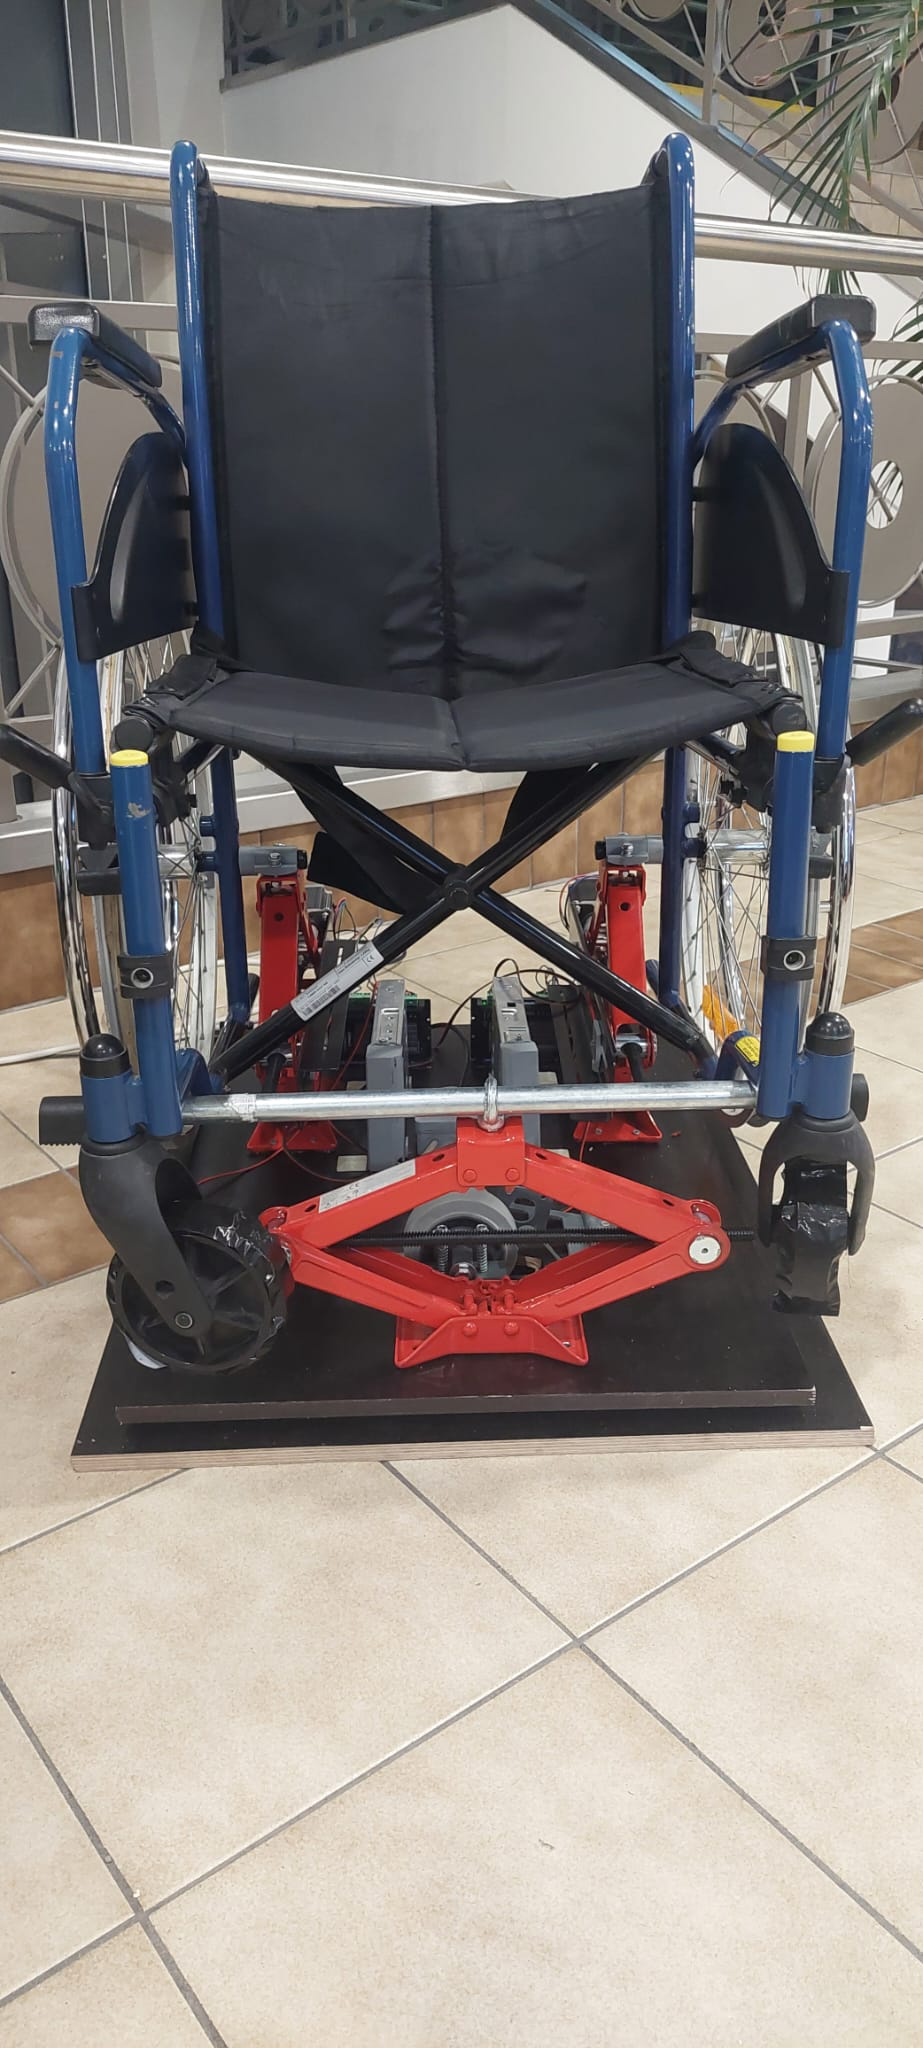
\includegraphics[scale=0.3]{pics/prototyp-ende.jpg}
    \caption{Prototyp Ende 21. November}
    \label{fig:prototyp-ende}
\end{figure}


\subsection{Motorenfindung: Schrittmotoren vs. Hydraulik}
\setauthor{Elisa Kaltenberger}

Hydrauliksysteme arbeiten mit Flüssigkeiten unter Druck, um signifikante Kräfte zu generieren. 
Die Verdrängung von Hydrauliköl durch einen Kolben ermöglicht die Erzeugung eines hohen Drucks, 
der die Bewegung schwerer Lasten oder präziser mechanischer Bewegung ermöglicht.

Derartige Systeme erweisen sich als vorteilhaft, wenn es darum geht, große Kräfte, Drehmomente oder 
schwere Lasten zu bewegen. Dies ist beispielsweise in Baumaschinen, Hebebühnen oder bei Pressen der 
Fall.

Allerdings sind hydraulische Anlagen in der Regel durch eine komplexe Konstruktion charakterisiert, 
die Zylinder, Pumpen und eine Ölfüllung umfasst. Dies impliziert hohe Wartungsaufwendungen, eine 
aufwändige Installation sowie eine eingeschränkte Flexibilität, insbesondere in Bezug auf feinfühlige 
oder kontrollierte Bewegungen.

Sofern die betreffende Anwendung keine extrem schweren Lasten bewegt, sondern eher präzise, kontrollierte 
und wiederholbare Bewegung erfordert, ist eine Hydraulik-Lösung oft zu aufwändig.

Ein Schrittmotor hingegen ist ein bürstenloser Gleichstrommotor, dessen Rotationsbewegung nicht 
kontinuierlich, sondern in vorgegebenen und gleichmäßigen Schritten erfolgt.

Die Position lässt sich dadurch mit hoher Präzision, Reproduzierbarkeit und ohne zusätzliche Rückführung 
bestimmen. Dies ist vorteilhaft, wenn eine exakte Positionierung oder punktgenaue Steuerung erforderlich ist.

Die Realisierung von sehr feinen Schritten ist durch den Einsatz von Mikroschritt-Antrieben möglich, 
wodurch die Bewegungen nahezu glatt und servo-ähnlich wirken, ohne dass ein geschlossener Regelkreis 
erforderlich ist.

Darüber hinaus zeichnen sich Schrittmotoren im Vergleich zu hydraulischen Systemen durch eine kompakte 
Bauweise, ein geringes Gewicht, eine einfache Handhabung und Wartung aus. Es besteht keine Notwendigkeit 
für eine Ölversorgung, hydraulische Leitungen oder Zylinder, was Platz, Aufwand und potenzielle Fehlerquellen 
reduziert. 

Zusätzlich sind Schrittmotoren insbesondere dann sinnvoll, wenn die Anwendung häufige, gleichförmige oder 
wiederholbare Bewegungen erfordert, wie sie beispielsweise bei der Indexierung, Positionierung oder 
automatisierten Abläufen auftreten, und die Last gleichmäßig und vorhersehbar ist.

\subsection{Bauprozess}
Nachdem entschieden worden war, welche Antriebsart verwendet werden sollte, wurden die Motoren bestellt. 
Während der Lieferzeit machte man sich Gedanken darüber, wie die Konstruktion des Prototyps aussehen könnte. 
Die Überlegung war, auf einer Holzplatte eine zweite Platte zu montieren, die mithilfe von Rollen auf der 
unteren Platte beweglich ist. An der Unterseite dieser oberen, horizontal beweglichen Platte wurden kleine 
Rollen befestigt, die die horizontale Bewegung ermöglichen.

Zusätzlich wurde in die obere Holzplatte ein längliches Loch gefräst, sodass ein größeres Gummirad 
darin Platz findet. Dieses Rad ermöglicht die eigentliche horizontale Drehbewegung. Das Gummirad wurde 
anschließend mithilfe eines selbst gefertigten 3D-gedruckten Bauteils auf der oberen Platte befestigt 
(siehe Abb. 5: Befestigung des Gummirads). 

Das 3D-Teil wurde in KiCad konstruiert und in der Schule im Keller gedruckt. Es wurde dem Filament 
ABS gedruckt. Es wurde Acrylnitril-Butadien-Styrol (ABS) gewählt, denn es zeichnet sich durch eine 
hohe Steifigkeit, 
Zähigkeit und Festigkeit aus. Das Material zeichnet sich durch eine hohe Schlag- und Kratzfestigkeit 
aus und weist eine hohe Resilienz gegenüber mechanischen Belastungen auf. Zudem ist ABS beständig 
gegenüber Ölen, Fetten und vielen Chemikalien. Es weist eine gute Temperaturbeständigkeit auf und 
bleibt auch bei höheren Temperaturen formstabil. Außerdem lässt sich ABS vielseitig verarbeiten und 
gut nachbearbeiten, beispielsweise durch Schleifen oder Lackieren.
(Quelle 11)

\begin{figure}
    \centering
    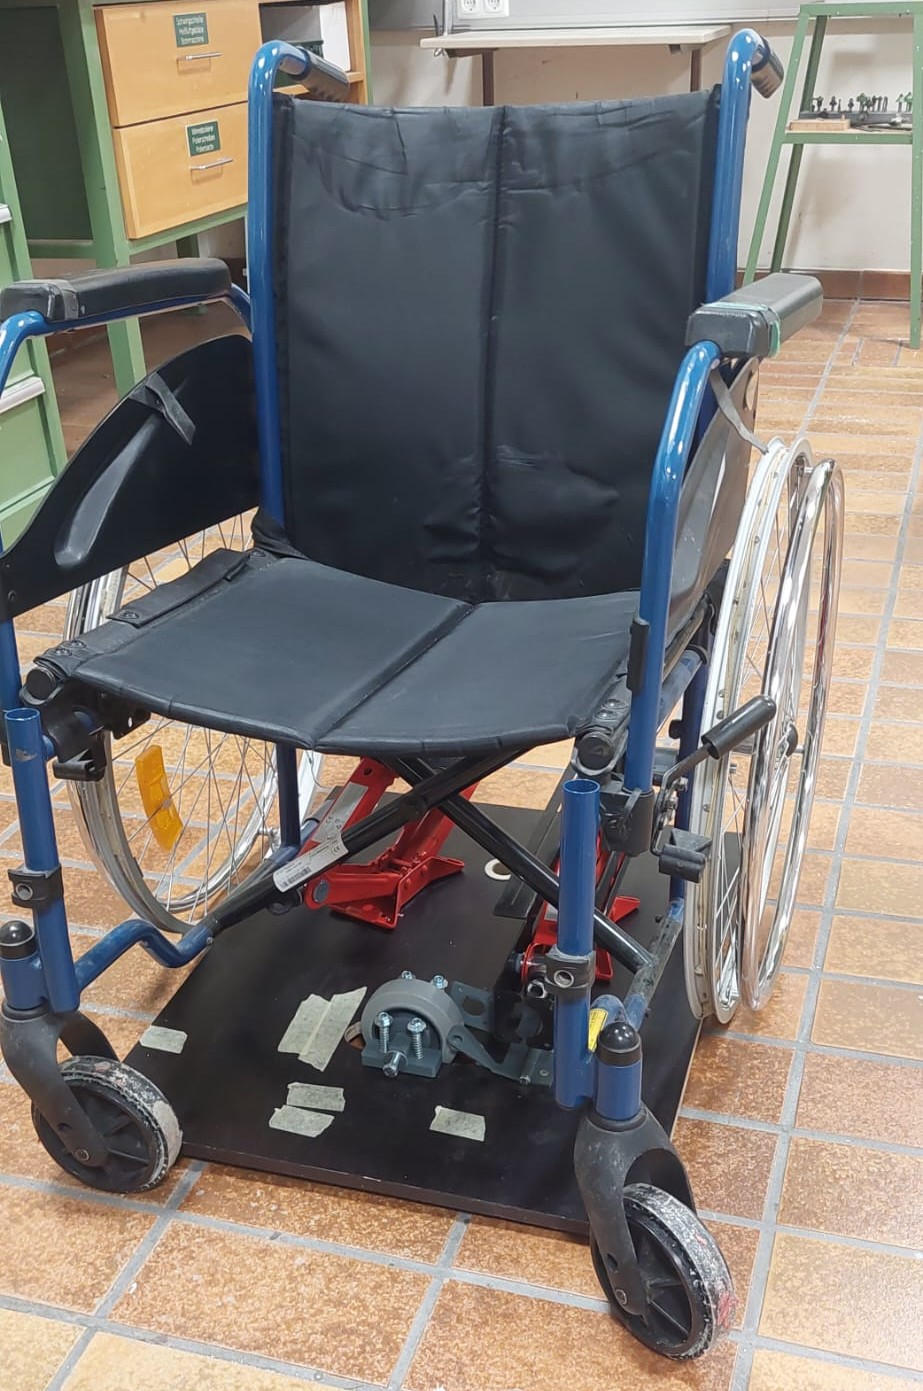
\includegraphics[scale=0.3]{pics/prototyp-zwischenstand.jpg}
    \caption{Prototyp Zwischnstand 13. November}
    \label{fig:prototyp-zwischenstand}
\end{figure}

Nachdem alles angeschraubt wurde, wurden die Wagenheber provisorisch positioniert, um einen ersten 
Eindruck von den Prototypen zu gewinnen, siehe Abb. \ref{fig:prototyp-zwischenstand}.

\subsection{Fertigung der Platine}
\setauthor{Elisa Kaltenberger}
Die Fertigung der Platine stellt einen zentralen Bestandteil des gesamten Entwicklungsprozesses dar 
und bildet die Grundlage für die zuverlässige Funktion der elektronischen Schaltung. Von der ersten 
Konzeption über die Layoutgestaltung bis hin zur eigentlichen Herstellung erfordert dieser Prozess 
ein präzises und systematisches Vorgehen. Sowohl die sorgfältige Planung mit geeigneten 
Entwicklungswerkzeugen als auch die fachgerechte Durchführung der einzelnen Fertigungsschritte 
tragen maßgeblich zur Qualität, Betriebssicherheit und Langlebigkeit der Leiterplatte bei.

Im Folgenden werden zunächst die Entwurfsphase der Leiterplatte sowie anschließend der technische 
Aufbau und die einzelnen Schritte des Herstellungsprozesses detailliert beschrieben.

\subsection{Layout in KiCad}
\setauthor{Elisa Kaltenberger}
Vor Beginn des eigentlichen Herstellungsprozesses wurde die Leiterplatte mithilfe von KiCad 
vollständig geplant und vorbereitet. Im ersten Schritt erfolgte die Erstellung eines detaillierten 
Schaltplans. Darin wurden sämtliche elektronischen Komponenten, einschließlich ihrer elektrischen 
Verbindungen, systematisch erfasst und eindeutig definiert. Der Fokus lag dabei auf einer klar 
strukturierten Darstellung, einer logisch aufgebauten Verschaltung sowie einer durchdachten Auswahl 
geeigneter Bauteile im Hinblick auf Funktionalität, Verfügbarkeit und elektrische Belastbarkeit.

Nach der sorgfältigen Überprüfung und Finalisierung des Schaltplans Abb.\ref{fig:schaltplan} wurde das Projekt in den 
Platinen-Editor von KiCad übertragen. Dort begann die konkrete Layoutgestaltung der Leiterplatte. 
Zunächst wurden alle Bauteile unter Berücksichtigung funktionaler Zusammenhänge sinnvoll auf der 
Leiterplatte positioniert. Ziel war es, kurze Signalwege zu ermöglichen, kritische Leitungen zu 
trennen und eine möglichst übersichtliche Anordnung zu schaffen. Auch mechanische Aspekte, wie 
Befestigungspunkte oder spätere Einbaumöglichkeiten, wurden dabei berücksichtigt.

\begin{figure}
    \centering
    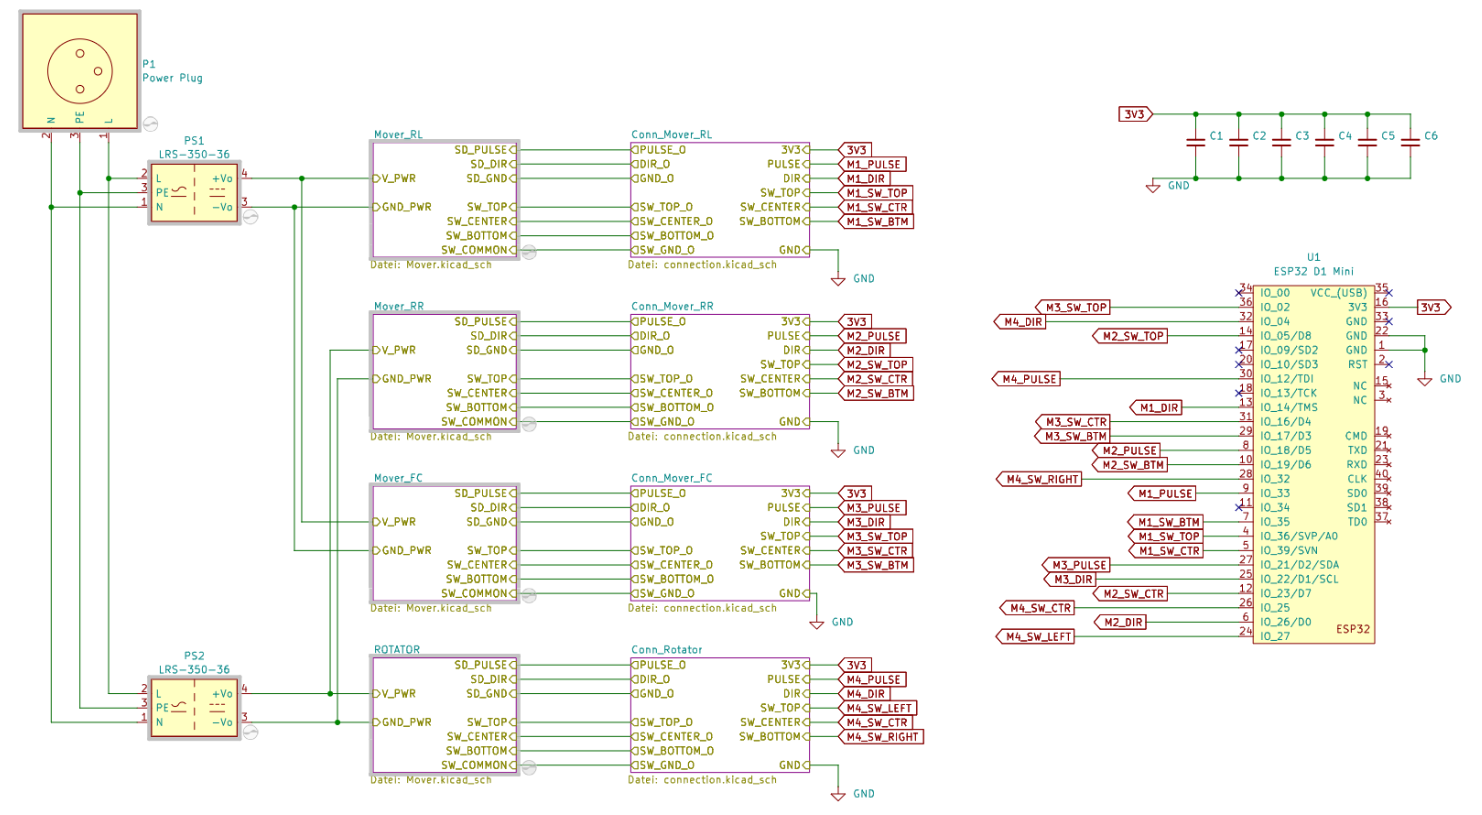
\includegraphics[scale=0.5]{pics/Schaltplan.png}
    \caption{Schaltplan der Platine}
    \label{fig:schaltplan}
\end{figure}

Im nächsten Schritt erfolgte das Routing der Leiterbahnen. Hierbei wurde darauf geachtet, 
Signalstörungen zu minimieren, Kreuzungen möglichst zu vermeiden und eine saubere, nachvollziehbare 
Leitungsführung zu gewährleisten. Versorgungsleitungen wurden entsprechend dimensioniert, während 
empfindliche Signalleitungen mit besonderer Sorgfalt behandelt wurden. Zusätzlich wurden sämtliche 
Designregeln, wie Mindestabstände zwischen Leiterbahnen, geeignete Leiterbahnbreiten sowie Vorgaben 
für Durchkontaktierungen, konsequent eingehalten. Abschließend wurde das Layout nochmals überprüft, 
um mögliche Fehler frühzeitig zu erkennen und eine reibungslose Fertigung der Platine sicherzustellen.

\subsection{Platinenherstellung}
\setauthor{Elisa Kaltenberger}
Bei der Herstellung von Leiterplatten kommt dem konstruktiven Aufbau sowie der präzisen Abstimmung 
der einzelnen Fertigungsschritte eine entscheidende Bedeutung zu. Diesbezüglich sind insbesondere die 
spätere Funktionalität, Lebensdauer und Betriebssicherheit zu berücksichtigen. Bereits geringfügige 
Abweichungen im Prozess können die elektrische Leitfähigkeit, die mechanische Stabilität oder die 
Lötqualität erheblich beeinflussen.

Eine typische Leiterplatte besteht im Wesentlichen aus mehreren aufeinander abgestimmten Schichten. 
Die Grundlage bildet das Basismaterial, häufig ein glasfaserverstärktes Epoxidharz. Dieses dient als 
mechanische Trägerstruktur und sorgt gleichzeitig für die notwendige elektrische Isolation zwischen 
den leitenden Strukturen. Auf dieses Substrat wird eine dünne Kupferschicht aufgebracht beziehungsweise 
auflaminiert. Sie stellt das eigentliche leitfähige Material dar, aus dem später die Leiterbahnen, 
Masseflächen und Kontaktpads entstehen. Abschließend wird die Oberfläche mit einer lichtempfindlichen 
Fotolackschicht versehen. Diese fungiert als temporäre Schutz- und Maskierungsschicht, mit deren Hilfe 
das gewünschte Leiterbild präzise übertragen werden kann.

Der eigentliche Fertigungsprozess erfolgt in mehreren aufeinander abgestimmten Schritten. Zu Beginn des 
Verfahrens wird die mit Fotolack beschichtete Kupferfläche mittels UV-Licht belichtet. Hierbei wird eine 
Belichtungsvorlage verwendet, welche die späteren Leiterbahnen abbildet. An den belichteten Stellen erfolgt 
eine Aushärtung des Fotolacks, wodurch eine chemische Beständigkeit des Materials gewährleistet wird. Die 
unbelichteten Bereiche bleiben hingegen löslich.

Darauf folgt die Entwicklung der Platine in einer geeigneten Entwicklerlösung, die häufig auf Basis von 
Natronlauge basiert.  In diesem Schritt werden die nicht ausgehärteten Fotolackanteile entfernt, wodurch das 
darunterliegende Kupfer freigelegt wird. Das gewünschte Leiterbild wird dadurch erstmals sichtbar, da nur 
die durch den gehärteten Fotolack geschützten Bereiche erhalten bleiben.

Im darauffolgenden Ätzprozess wird das freiliegende, ungeschützte Kupfer unter Einsatz spezifischer Ätzmittel 
einer chemischen Reaktion unterzogen, die zu dessen Abtrag führt. Das Kupfer ist das einzige Element, das nach 
der Behandlung übrig bleibt und zuvor durch den gehärteten Fotolack geschützt wurde. Diese bilden nun die 
endgültigen Leiterbahnen der Schaltung. Je nach Aufbau der Platine können danach zusätzliche Arbeitsschritte 
wie das Bohren von Bauteil- und Durchkontaktierungslöchern erfolgen. Bei mehrlagigen Leiterplatten werden 
diese Bohrungen metallisiert, um elektrische Verbindungen zwischen verschiedenen Kupferschichten herzustellen.

Nach dem Ätzvorgang wird der verbliebene Fotolack im sogenannten Entschichtungsprozess vollständig entfernt. 
Die Kupferoberflächen werden gereinigt und gegebenenfalls chemisch nachbehandelt, um eine optimale 
Weiterverarbeitung zu gewährleisten. Im darauffolgenden Schritt wird die Lötstoppmaske aufgebracht. Diese 
Schutzschicht bedeckt nahezu die gesamte Leiterplatte und lässt lediglich die Lötpads frei. Sie schützt die 
Leiterbahnen vor Oxidation, verhindert ungewollte Lötbrücken und verbessert die elektrische sowie mechanische 
Zuverlässigkeit.

Nachdem alle Schritte der Platinenherstellung erfolgreich abgeschlossen wurden Abb. \ref{fig:platine}, 
wurden LEDS und Wiederstände auf der Platine verlötet. Es wurden LEDs und Widerstände verbaut, um die 
Funktionalität der Platine zu gewährleisten. Die LEDs dienen als visuelle Indikatoren für den Betriebszustand 
der Schaltung, während die Widerstände den Stromfluss regulieren und somit die Bauteile vor Überlastung 
schützen. Die sorgfältige Auswahl und Anordnung dieser Komponenten auf der Platine tragen maßgeblich zur 
Stabilität und Zuverlässigkeit der elektronischen Schaltung bei.
(Quelle 12 bis 16)

\begin{figure}
    \centering
    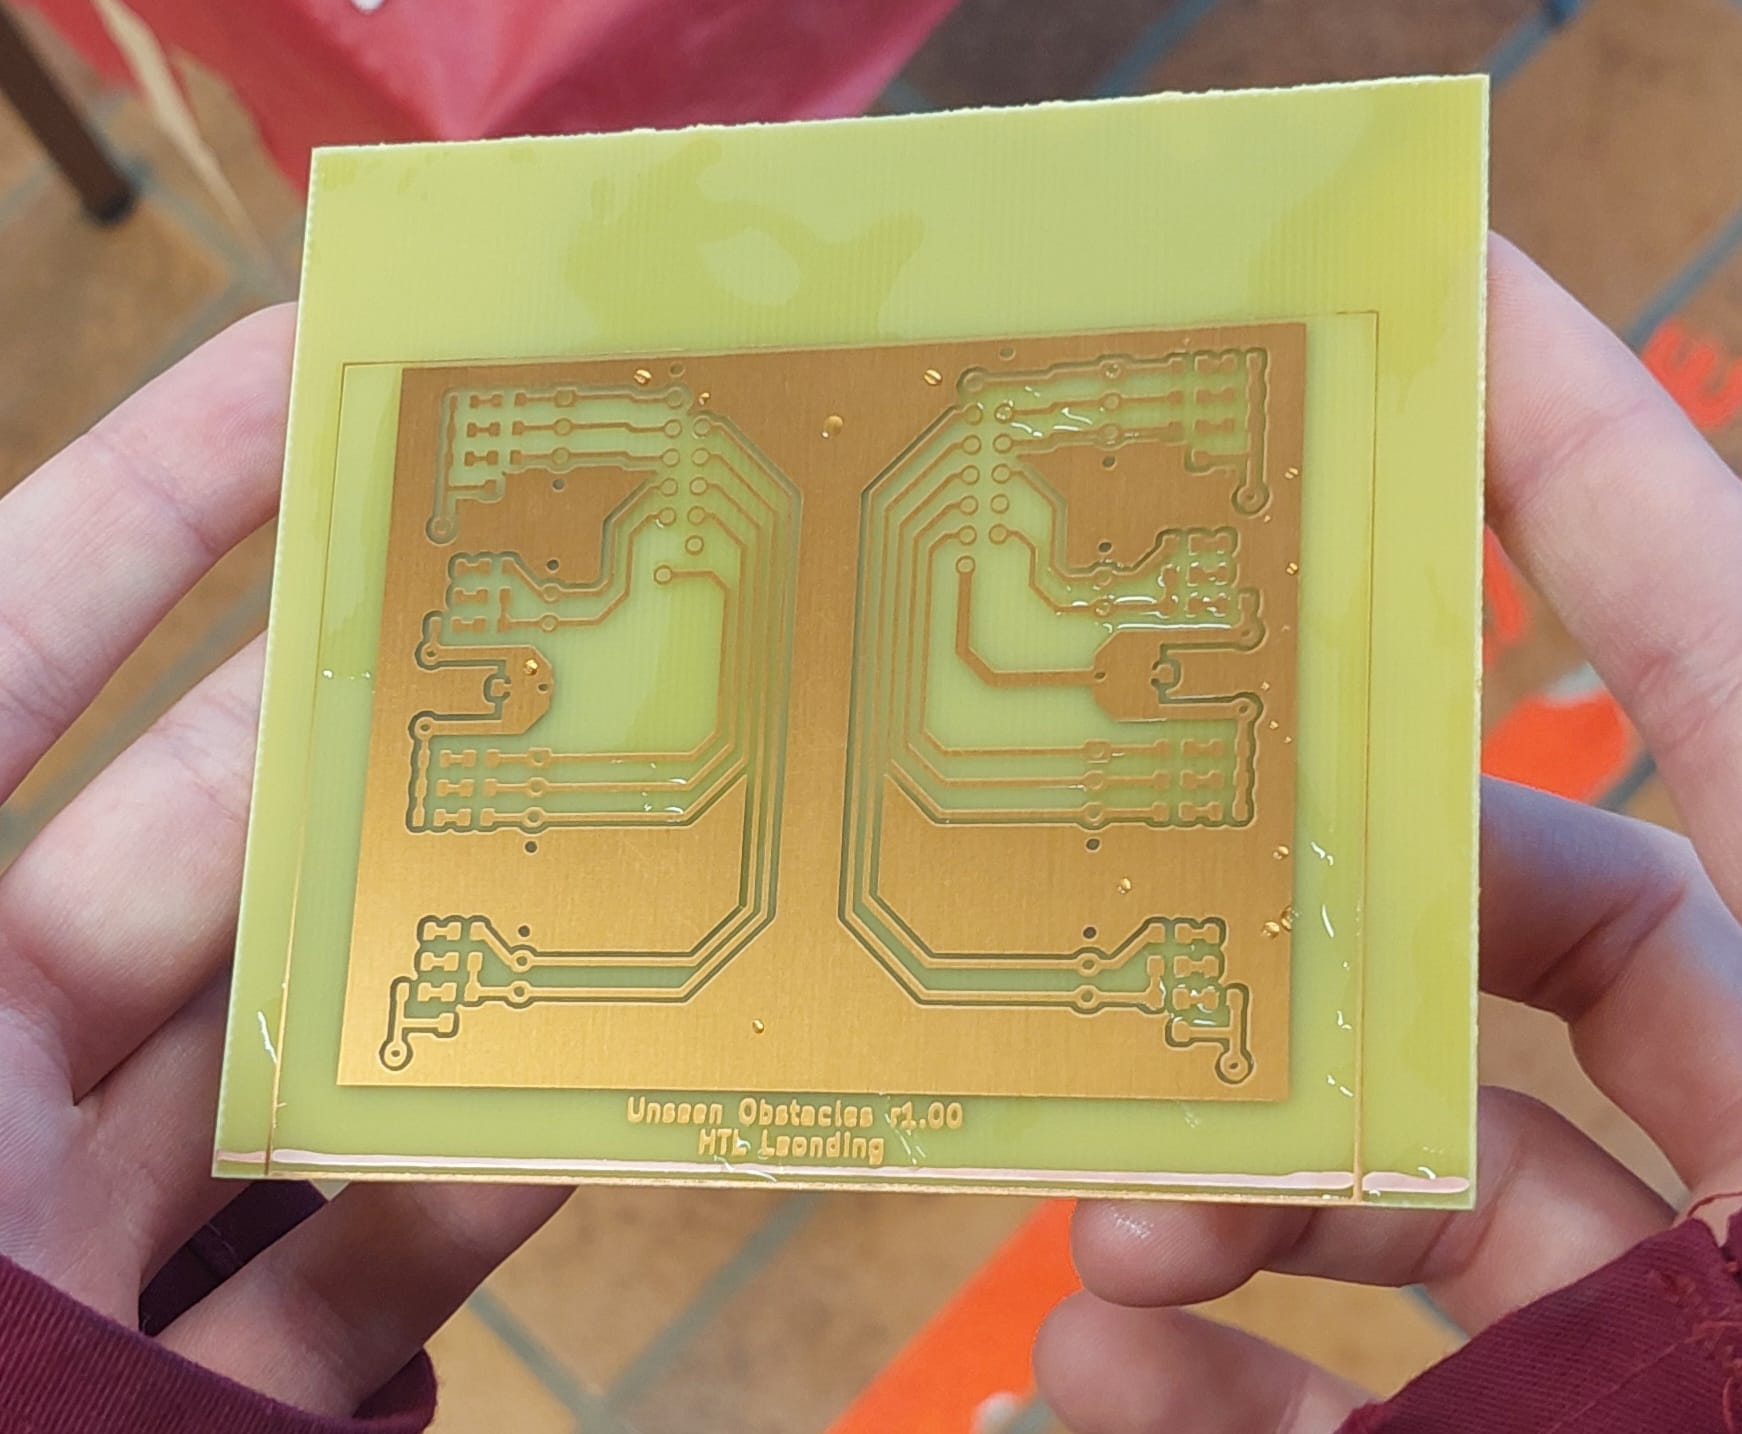
\includegraphics[scale=0.2]{pics/platine.jpg}
    \caption{Platine Prototyp}
    \label{fig:platine}
\end{figure}


\begin{spacing}{1}
\chapter{Kommunikation zwischen Hardware-Simulator und VR-Simulation}\label{chapter:communication_vr_hardware}
\end{spacing}
Die Kopplung des physischen Hardware-Prototyps mit der virtuellen Simulationsumgebung konstituiert einen zentralen Bestandteil des Projekts. Insbesondere im Kontext von Virtual-Reality-Anwendungen ermöglicht die Integration realer Eingabegeräte mit virtuellen Systemmodellen eine realitätsnahe Interaktion sowie die Untersuchung von Systemverhalten unter kontrollierten Bedingungen.

Eine zentrale Herausforderung bei der Implementierung solcher hybrider Systeme besteht in der zuverlässigen und latenzarmen Kommunikation zwischen der Hardwarekomponente und der VR-Anwendung. Um eine konsistente Abbildung des physischen System innerhalt der virtuellen Umgebung zu gewährleisten, ist ein kontinuierlicher Austausch von Zustands- und Steuerdaten erforderlich. Dabei spielen Aspekte wie die Datenformatierung, die Synchronisation der Systemzustände sowie die Minimierung von Übertragungs- und Verarbeitungszeiten eine entscheidende Rolle für die Gesamtperformance des Systems.

In diesem Abschnitt wird die Implementierung Kommunikationsarchitektur zwischen dem Hardwareprototyp und der VR-Simulation beschrieben. Zunächst erfolgt eine Erläuterung der grundlegenden Systemstruktur sowie der Rolle der einzelnen Komponenten. Im Anschluss erfolgt die Darstellung des verwendeten Kommunikationsmechanismus sowie des zugrunde liegenden Datenprotokolls. Abschließend werden die Implementierungsdetails der Schnittstelle sowie Maßnahmen zur Gewährleistung einer stabilen und konsistenten Datenübertragung erörtert. 

\section{Systemarchitektur des Gesamtsystems}
\setauthor{Linnea Schönbauer}

Hier grundlegender Aufbau des Systems
hardware prototyp Umgebung
steuerungssoftware C++
bissl noch vr simulation Unity, C sharp  hier halt mehr auf die Sprache eingehen 
kommunikationsschnittstelle zwischen beiden

Das System besteht aus zwei Hauptkomponenten: Dem physischen Hardwareprototypen und einer VR-Simulation die über eine gemeinsame Kommunikationsschnittstelle verbunden sind. 

Architekturabbildung

beschreiben:
welche komponenten existieren, welche Aufgaben haben sie, wie sind sie miteinander verunden

\section{Architektur des VR-Projekts}
\setauthor{Linnea Schönbauer}
Die virtuelle Simulation wurde unter Verwendung der Game Engine Unity realisiert. Unity ist eine weit verbreitete Entwicklungsumgebung zur Erstellung interaktiver 3D-Anwendungen und Virtual-Reality-Systeme. Dee Engine stellt eine integrierte Entwicklungsumgebung bereit, welche Werkzeuge zur Szenengestaltung, Physiksimulation, Skriptprogrammierung sowie zur Verwaltung komplexer Objektstrukturen umfasst.

Ein zentrales Merkmal der Architektur von Unity ist die objektorientierte Organisation der virtuellen Welt. In der vorliegenden Arbeit wird dargelegt, dass sämtliche Elemente einer Simulation als Objekte innerhalb einer Szene modelliert werden. Zudem wird erörtert, dass die Steuerung dieser Objekte über ein komponentenbasiertes System erfolgt. (QUELLE Unity Seite)

Unity organisiert alle Inhalte einer Simulation in sogenannten Szenen, die jeweils eine hierarchische Baumstruktur aus GameObjects bilden. Eine Szene konstituiert eine abgeschlossene virtuelle Umgebung, welche sämtliche geometrischen Objekte, Lichtquellen, Kameras sowie Interaktionskomponenten enthält.

Die Struktur innerhalt einer Szene folgt einer hierarchischen Organisation, in der einzelne GameObjects in Parent-Child-Beziehungen zueinander stehen können. Diese Struktur ermöglicht eine effiziente Verwaltung komplexer Objektsysteme, da Transformationen eines übergeordneten Objekts automatisch auf seine untergeordneten Elemente übertragen werden.

BEISPIEL ROLLSTUHL ALS CHILD OBJEKT DES XOR RIGS UND AUSSERDEM FOTO VON DER HIERARCHIE IN UNITY

In dem Computerspiel-Entwicklungsprogramm Unity wird jedes Element der virtuellen Welt als sogenanntes GameObject bezeichnet. GameObjects dienen als Container für verschiedene Komponenten, welche dsa Verhalten und die Eigenschaften des jeweiligen Objekts definieren. Ein GameObject verfügt anfänglich über keine Funktionalität sondern diese wird erst durch die hinzugefügten Komponenten erworben. 

Als illustrierende Beispiele für GameObjects innerhalt der Simulation seien etwa Gebäude der virtuellen Stadtumgebung, Straßenelemente, Kollisionsobjekte oder der virtuelle Rollstuhl genannt, der als zentrales Interaktionselement der Anwendung dient \ref{chapter:vr-world}. (QUELLE UNITY SEITE)

\subsection{Physikalisches Bewegungsmodell}
\setauthor{Linnea Schönbauer}
Die Bewegung des virtuellen Rollstuhls innerhalb der Simulation basiert auf der Physik-Engine der Game Engine Unity. Anstatt die Positionsänderungen direkt zu manipulieren, wird ein physikalisches Bewegungsmodell verwendet, das auf der sogenannten Rigidbody-Komponente basiert. (QUELLE RIGIDBODY)

Diese Komponente gestattet die Simulation physikalischer Eigenschaften wie Masse, Gravitation sowie Kollisionen mit anderen Objekten der virtuellen Umgebung. Dies resultiert in einem realistischeren Bewegungsverhalten, insbesondere beim Befahren von Steigungen oder beim Kontakt mit Hindernissen innerhalb der simulierten Stadtumgebung.

Im Rahmen des vorliegenden Systems wird der virtuelle Rollstuhl daher als physikalisches Objekt modelliert, dessen Position und Orientierung über die Bewegungsfunktionen der Rigidbody-Komponente gesteuert werden. 

\subsection{Positions- und Orientierungsparameter des virtuellen Rollstuhls}
\setauthor{Linnea Schönbauer}
Die Simulation des virtuellen Rollstuhls erfolgt unter Verwendung von Positions- und Orientierungsdaten zur adäquaten Beschreibung der Bewegung innerhalb der Simulation. Diese Werte beschreiben den aktuellen Zustand des Objekts im dreidimensionalen Raum und bilden gleichzeitig die Grundlage für die spätere Übertragung an den Hardwareprototyp.

\subsubsection{Positionskoordinaten}
\setauthor{Linnea Schönbauer}
Die Position eines Objekts in der Simulation wird durch ein kartesisches Koordinatensystem beschrieben. Die Position eines Objekts wird durch drei Koordinaten entlang der räumlichen Achse definiert.

Die Koordinate PosX beschreibt die Position entlang der horizontalen X-Achse, während PosZ die Bewegung entlang der Tiefenachse der virtuellen Umgebung angibt. Die vertikale Position wird durch PosY beschrieben und repräsentiert die Höhe des Objekts innerhalb der Szene.

\subsubsection{Orientierung im Raum}
\setauthor{Linnea Schönbauer}
Abgesehen von der Position ist auch die Orientierung des Rollstuhls im Raum von signifikanter Relevanz. Die vorliegende Beschreibung gibt Aufschluss über die Ausrichtung des Objekts relativ zu den drei Raumachsen.

In einer Vielzahl von 3D-Systemen wird diese Orientierung durch sogenannte Euler-Angles repräsentiert, welche drei Rotationswinkel entlang der Raumachsen definieren. (QUELLE)

BEISPIEL BILD VON DEM EULER FREIHEITSGRADE DIAGRAMM KREIS SPHERE QUELLE

\subsubsection{Pitch, Yaw und Roll}
\setauthor{Linnea Schönbauer}
Die Orientierung wird durch drei Rotationswinkel beschrieben, die jeweils eine Drehung um eine der Raumachsen repräsentieren.

Pitch beschreibt die Rotation um die seitliche Achse des Objekts und entspricht einer Vorwärts- oder Rückwärtsneigung. Das Befahren einer steilen Rampe führt beispielsweise zu einer signifikanten Änderung des Pitch.

Yaw beschreibt die Rotation um die vertikale Achse und determiniert damit die Blickrichtung des Rollstuhls innerhalb der Umgebung.

Roll beschreibt die seitliche Neigung des Objekts um die Vorwärtsachse. Ein Beispiel für eine derartige Situation wäre das Befahren eines hohen Bordsteins, wobei sich das Fahrzeug mit einem Reifen auf dem Gehweg und mit dem anderen auf der Straße befindet.

\subsubsection{Freiheitsgrade des Systems}
\setauthor{Linnea Schönbauer}
Die Bewegung des Rollstuhls lässt sich somit durch sechs Freiheitsgrade beschreiben. Drei dieser Freiheitsgrade betreffen die Position des Objekts im Raum (Translation entlang der X-, Y- und Z-Achse), während die übrigen drei Freiheitsgrade die Orientierung des Objekts beschreiben (Rotation um die drei Raumachsen).

\subsection{Verarbeitung der Benutzereingaben}
\setauthor{Linnea Schönbauer}
Die Steuerung des virtuellen Rollstuhls erfolgt durch Eingaben des Benutzers, welche durch das Input-System von Unity erfasst werden. Diese Eingaben werden als zweidimensionaler Eingabevektor interpretiert, der sowohl Vorwärtsbewegung als auch Rotationsbewegung repräsentiert.

Der vertikale Anteil des Eingabevektors determiniert die Vorwärts, beziehungsweise Rückwärtsbewegung des Rollstuhls innerhalb der Szene, während der horizontale Anteil zur Steuerung der Drehbewegung um die vertikale Achse verwendet wird.

Die vorliegende Aufteilung ermöglicht die unabhängige Kontrolle von Translation und Rotation, wodurch eine intuitive Navigation innerhalb der virtuellen Umgebung ermöglicht wird. (QUELLE bzw. Wiederholung von Kapitel Bewegung im virtuellen Raum)

\subsection{Berechnung der Translation und Rotation}
\setauthor{Linnea Schönbauer}
Die Bewegung des Rollstuhls lässt sich in zwei grundlegende Bewegungsarten unterteilen: Die translatorische Bewegung entlang der Blickrichtung sowie die Rotationsbewegung um die vertikale Achse.

Die Berechnung der Vorwärtsbewegung erfolgt entlang der lokalen Vorwärtsrichtung des Rollstuhls. Diese Richtung entspricht der aktuellen Orientierung des Rollstuhls innerhalb der Szene und wird über die Transformationsdaten des Objekts bestimmt. Die tatsächliche Verschiebung pro Simulationsschritt ergibt sich demnach aus der definierten Bewegungsgeschwindigkeit sowie der Zeitdauer des jeweiligen Physiks-Updates.

Darüber hinaus besteht die Möglichkeit, den Rollstuhl um die vertikale Achse zu rotieren, wodurch Richtungsänderungen innerhalb der virtuellen Umgebung ermöglicht werden. Die Rotationsgeschwindigkeit wird über einen separaten Parameter gesteuert und ebenfalls innerhalb des Physik-Update-Zyklus der Simulation berechnet. (QUELLE CODE?)




\section {Datenaustausch zwischen Simulation und Hardware}
\setauthor{Linnea Schönbauer}
hier erklären welche daten zwischen simulation und hardware übertragen werden.
z.b. halt das pitch, yaw, roll, etc. position, und halt auch wie man das aus der simulation kriegen

außerdem beschreiben: datenformat, übertragunsgfrequenz, kommunikationsprotokoll also das ganze udp beschreiben und auch mit app und so


\section{Steuerungslogik und Regelkreis}
\setauthor{Linnea Schönbauer}
hier beschreiben wie die Simulation Bewegungsbefehle generiert und wie die hardware darauf reagiert:

ablauf eventuell:
simulation berechnet einen neuen Zustand
zielposiition oder bewegungsbefehl wird erzeugt
befehl wird an den hardwarecontroller übertragen
hardware führt bewegung aus
sensoren liefern feedback (also sie erheben sich die heber)
simulation wird aktualisiert

das ist geschlossener Regelkreis hier kann man auch skizze einfügen Immersion

Buzzwords: Control Loop, Feedback Loop, Regelkreis

\section{Synchronisation zwischen Simulation und Hardware}
\setauthor{Linnea Schönbauer}
hier beschreib das problem dass simulation und hardware oft mit unterschiedlichen aktualisierungsraten arbeiten also vr rendering oft 90 hz und hardware steuerung oft 100 hz.

führt potentiell zu:
positionsabweichungen, verzögerungen, instabile Bewegungen

deshalb werden synchronisationsmethoden verwendet, z.B.:
zeitstempel, interpolation, vorhersagemodelle

\section{Latenz und Echtzeitanforderungen}
\setauthor{Linnea Schönbauer}
Hier erklären warum niedrige Latenz wichtig ist.

In VR-Systemen entsteht Verzögerung durch:
sensordatenerfassung, Datenübertragungn, Verarbeitung, Renderkng, Hardwarebewegung

Diese gesamte Verzögerung wird oft Motion-to-Photon-Latenz genannt. 

Zu hohe Latenz kann dazu führen dass:
Bewegungen nicht synchron erscheinen, Interaktionen unnatürlich wirken, Systeminstabilität entsteht

\section{Hardware-in-the-Loop Integration}
\setauthor{Linnea Schönbauer}
Hier kann man system theoretisch Einordnen 

wahrscheinlich sit projekt hardware-in-the-loop system. Das heißt ein reales Hardwaregerät ist Teil einer Simulation. Simulation und Hardware beeinflussen sich gegenseitig bzw. eigentlich nur die simulation die hardware.
Die simulation berechnet umgebung, bewegungen. Die Hardware führt reale Bewegungen aus.

\section{Abbildung der Simulationsbewegungen auf die Hardware}
\setauthor{Linnea Schönbauer}
hier wird dann der kernpunkt des Bulletpoints erklärt. Wie sich die Hardware entsprechend der Simulation bewegt

Typischer Ablauf:
Simulation berechnet zielzustand. also in dem fall position und yaw und pitch etc.

transformation in das koordinatensystem der hardware
berechnungn von steuerbefehlen also motorposition, aktuatorsteuerung,
 (hier auch code snippets von den calculations in mover driver? und die eine sizze von wenns auf am berg steht einfügen)
hardware führt bewegung aus

\section{Implementierungsdetails}
\setauthor{Linnea Schönbauer}
ughhh keine Ahnung nochmal alles zusammenfassen maybe

\begin{spacing}{1}
\chapter{Gestalterische Elemente zur Förderung der Immersion}\label{chapter:immersion}
\end{spacing}
Die vorliegende Simulation zielt darauf ab, die Herausforderungen, mit denen Rollstuhlnutzerinnen und Rollstuhlnutzer im urbanen Raum konfrontiert sind, so realitätsnah und nachvollziehbar wie möglich darzustellen. Neben der technischen Realisierung der Bewegungsplattform ist auch die Gestaltung der virtuellen Umgebung von entscheidender Bedeutung. Virtuelle Realitäten entfalten ihre Wirkung insbesondere dann, wenn Nutzende das Gefühl entwickeln, sich tatsächlich innerhalb der dargestellten Umgebung zu befinden. Dieses Empfinden wird in der Forschung häufig als Immersion bezeichnet (QUELLE)

Um eine solche immersive Erfahrung zu ermöglichen, müssen verschiedene gestalterische und konzeptionelle Aspekte berücksichtigt werden. Zu den relevanten Faktoren zählen demnach eine klare Nutzerführung, eine verständliche Informationsvermittlung, eine realitätsnahe audiovisuelle Gestaltung sowie eine strukturierte Präsentation der Inhalte innerhalb der Simulation. Im Rahmen des Projekts wurde daher mehrere Gestaltungselemente entwickelt, die darauf abzielen, die Orientierung der Nutzenden zu erleichtern und gleichzeitig ein möglichst realistisches Erlebnis der simulierten Umgebung zu ermöglichen. (QUELLE)

\section{Nutzerführung und Einführung in die Simulation}
\setauthor{Linnea Schönbauer}
Zu Beginn der Simulation erfolgt die Einführung der Nutzenden in die Anwendung über einen Startbildschirm. Der Startscreen ist ein elementarer Bestandteil der Simulation, dessen Funktionalität sich aus der Interaktion mit weiteren Elementen der Simulation ergibt. Einerseits dient er der kurzen inhaltlichen Einordnung des Projekts, indem er den Zweck der Simulation erläutert und den Nutzenden eine grundlegende Orientierung über den Ablauf vermittelt. Andererseits markiert der den Ausgangspunkt der eigentlichen Simulation. (QUELLE)

Die Integration eines solchen Einstiegsbildschirms ist insbesondere in interaktiven Anwendungen von Relevanz, da Nutzende ohne vorausgegangene Erklärung häufig Schwierigkeiten haben können, den Kontext der Simulation oder ihre eigene Roll innerhalb der virtuellen Umgebung zu verstehen. Die kurze textliche Einführung zu Beginn der Simulation dient dazu, den Nutzenden bereits vor dem Beginn der Anwendung einen Überblick über die zu erwartenden Erfahrungen zu verschaffen. (QUELLE)

\begin{spacing}{1}
\chapter{Zusammenfassung}
\end{spacing}
Zusammenfassend lässt sich festhalten, dass im Rahmen dieser Arbeit erfolgreich eine immersive Virtual-Reality-Anwendung zur Simulation der Fortbewegung im Rollstuhl entwickelt wurde. Das Ziel bestand darin, Barrieren im urbanen und baulichen Umfeld erfahrbar zu machen und das Bewusstsein für die Herausforderungen von Rollstuhlfahrenden zu stärken.

Die Ergebnisse zeigen, dass insbesondere die Kombination aus virtueller Umgebung und physischer Simulation durch den entwickelten Hardware-Simulator ein intensives und realistisches Nutzererlebnis ermöglicht. Die Integration von haptischem Feedback, wie Neigung und Vibrationen, trägt wesentlich zur Immersion bei und hebt die Anwendung von herkömmlichen VR-Systemen ab.

Zukünftige Arbeiten könnten sich auf die Weiterentwicklung der Hardware, die Erweiterung der simulierten Szenarien sowie die Durchführung umfangreicher Nutzerstudien zur Evaluation der Wirkung konzentrieren.
Darüber hinaus empfiehlt es sich, die virtuelle Realität um eine größere Vielfalt an Hindernissen und Interaktionselementen zu erweitern, um eine noch realitätsnähere und anspruchsvollere Umgebung zu schaffen. In diesem Zusammenhang sollten diese zusätzlichen Hindernisse auch in die Hardware-Simulation integriert werden, sodass sie nicht nur visuell, sondern ebenfalls physisch korrekt erfahrbar sind und demnach eine konsistente Abbildung der virtuellen Umgebung gewährleistet wird.

\newpage
\pagenumbering{Roman}
\setcounter{page}{\value{RPages}}
\input{glossary}
%\setlength{\glsdescwidth}{0.8\linewidth}
\glsnogroupskiptrue
\IfStrEq{\thesislang}{de}
{
	\printglossary[title=Glossar,toctitle=Glossar] %,style=long]
}
{
	\printglossary[title=Glossary,toctitle=Glossary] %,style=long]
}
\spacing{1}{
\IfStrEq{\thesislang}{de}
{
	\bibliographystyle{ieeetrande}
}
{
	\bibliographystyle{IEEEtran}
}
\bibliography{bib}
}
\listoffigures
\listoftables
\lstlistoflistings
\appendix
\addchap{Anhang}
\input{./sections/appendix}
\end{document}

